\documentclass [aspectratio=169]{beamer}
\usepackage{listings}
\usepackage{enumitem}
\usepackage[T5]{fontenc}
\usepackage[utf8]{inputenc}
\beamertemplatenavigationsymbolsempty
\usetheme{Boadilla}
\usepackage{textpos} % package for the positioning
\usepackage[]{graphicx}
\usepackage{graphicx}
\usepackage{float}
\usepackage{hyperref}
\usepackage{caption}
\usepackage{subcaption}
\usepackage{algorithm,algpseudocode}
\usepackage[export]{adjustbox}
\usepackage{tikz}
\usepackage[square,numbers]{natbib}
\usepackage[byname]{smartref}
\usetikzlibrary{positioning}
\usetikzlibrary{arrows, shapes, decorations, automata, backgrounds, fit, petri, calc}
\usepackage{tikz}
\usetikzlibrary{arrows.meta, positioning}
\definecolor{blue}{RGB}{173,216,230}
\definecolor{green}{RGB}{144, 238, 144}
\newcommand*{\logofont}{\fontfamily{phv}\selectfont}

\definecolor{uwopurple}{RGB}{79,38,131} % official purple color for uwo

\title[]{\vspace{60pt} \\
Dysarthria and Non-Dysarthria Speech Classification} % Change the lecture topic right here!
%\subtitle{n}
\author[]{Vo Tran Hien - Pham Minh Duc - Vu Mai Thuy - Nguyen Dang Huu Thinh}
\institute[]{University of Science, Viet Nam National University, HCMC\\
             Faculty of Information Technology}
\date{\today}

% Math notations
\newtheorem{thm}{Theorem}[section]
\newtheorem{lem}[thm]{Lemma}

\newtheorem{defn}[thm]{Definition}
\newtheorem{eg}[thm]{Example}
\newtheorem{ex}[thm]{Exercise}
\newtheorem{conj}[thm]{Conjecture}
\newtheorem{cor}[thm]{Corollary}
\newtheorem{claim}[thm]{Claim}
\newtheorem{rmk}[thm]{Remark}

\newcommand{\ie}{\emph{i.e.} }
\newcommand{\cf}{\emph{cf.} }
\newcommand{\into}{\hookrightarrow}
\newcommand{\dirac}{\slashed{\partial}}
\newcommand{\R}{\mathbb{R}}
\newcommand{\C}{\mathbb{C}}
\newcommand{\Z}{\mathbb{Z}}
\newcommand{\N}{\mathbb{N}}
\newcommand{\Q}{\mathbb{Q}}
\newcommand{\LieT}{\mathfrak{t}}
\newcommand{\T}{\mathbb{T}}
\newcommand{\A}{\mathds{A}}
\newcommand{\E}{\mathbb{E}}
\newcommand{\Prob}{\mathbb{P}}
\newcommand{\Var}{\text{Var}}
\newcommand\equalhat{%
\let\savearraystretch\arraystretch
\renewcommand\arraystretch{0.3}
\begin{array}{c}
\stretchto{
    \scalerel*[\widthof{=}]{\wedge}
    {\rule{1ex}{3ex}}%
}{0.5ex}\\ 
=%
\end{array}
\let\arraystretch\savearraystretch
}

% set color
\setbeamercolor{title in head/foot}{bg=white}
\setbeamercolor{author in head/foot}{bg=white}
\setbeamercolor{date in head/foot}{fg=uwopurple}
\setbeamercolor{date in head/foot}{bg=white}
\setbeamercolor{title}{fg=uwopurple}
\setbeamerfont{title}{series=\bfseries}
\setbeamercolor{frametitle}{fg=uwopurple}
\setbeamerfont{frametitle}{series=\bfseries}
\setbeamercolor{block title}{bg=uwopurple!30,fg=black}
\setbeamercolor{item}{fg=uwopurple}
\setbeamercolor{caption name}{fg=uwopurple!70!}





% set logo at non-title pages
\logo{
\includegraphics[height=0.9cm]{im.jpg}\vspace*{-.055\paperheight}\hspace*{.85\paperwidth}}

\begin{document}

{
\setbeamertemplate{logo}{}
\begin{frame}
    \titlepage
    \begin{textblock*}{2cm}(2.5cm,-7.5cm)
        
\includegraphics[width=2cm]{im.jpg}
    \end{textblock*}
    \begin{textblock*}{8cm}(5.0cm,-7.0cm)
        \huge \color{uwopurple}{$\Bigr\rvert$ \hspace{0.15cm} \textbf{Group 09}} % Change the lecture # right here! 
    \end{textblock*}
\end{frame}
}

\section{Introduction}

\subsection{History}

\begin{frame}{History}
    \begin{itemize}[label=$\star$]
        \item The \textbf{Trie} data structure was first introduced by \textbf{René de la Briandais} in 1959 as an efficient method
for storing and retrieving strings in a lexicon
        \item It was later independently developed by \textbf{Edward
Fredkin} in 1960.
    \begin{figure}[h]
    \centering
    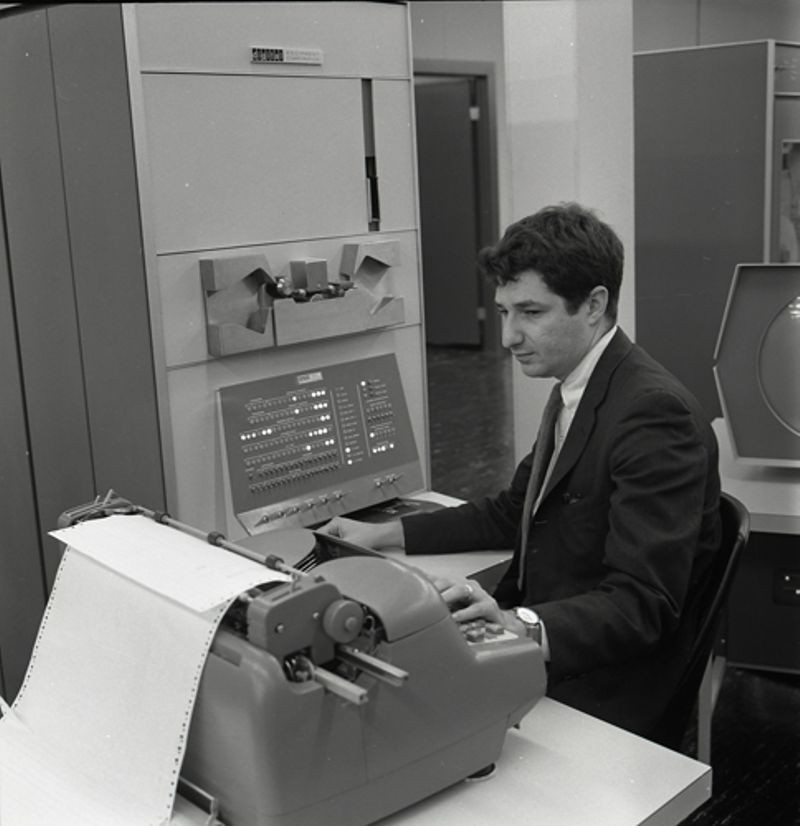
\includegraphics[scale=0.15]{EdSemi.jpg}
    \caption{Edward Fredkin}
    \label{fig:edsemi}
\end{figure}
    \end{itemize}
\end{frame}
\subsection{Definition}
\begin{frame}{Definition}
\textbf{A Trie} (also known as a \textbf{prefix tree}) is a tree-like data structure used to store a dynamic set or associative array where the keys are usually strings.
\begin{figure}[h]
    \centering
    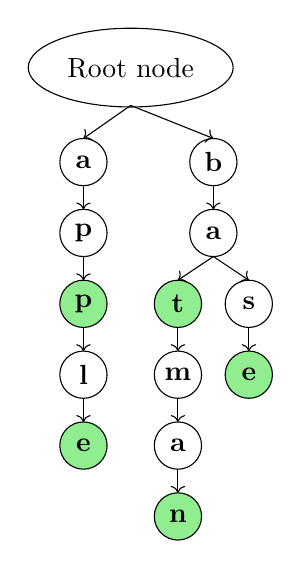
\begin{tikzpicture}[scale=0.6]
        % Vẽ hình elips chứa "Root node" tại tọa độ (0,0)
        \node[ellipse, draw, minimum width=2cm, minimum height=1cm] at (1,0) {Root node};
        
        % Vẽ vòng tròn chứa "a" tại (0,-2), không tô màu
        \fill[green] (0,-5) circle (0.5cm);
        \draw (0,-2) circle (0.5cm);
        \node at (0,-2) {\textbf{a}}; % Chữ "a" in đậm ở tâm vòng tròn
        \draw[->] (1,-0.8) -- (0,-1.5); % Mũi tên từ dưới "Root node" tới trên "a"
        
        % Vẽ vòng tròn chứa "p" thứ nhất tại (0,-3.5), không tô màu
        \draw (0,-3.5) circle (0.5cm);
        \node at (0,-3.5) {\textbf{p}}; % Chữ "p" in đậm ở tâm vòng tròn
        \draw[->] (0,-2.5) -- (0,-3); % Mũi tên từ dưới "a" tới trên "p"
        
        % Vẽ vòng tròn chứa "p" thứ hai tại (0,-5), không tô màu
        \draw (0,-5) circle (0.5cm);
        \node at (0,-5) {\textbf{p}}; % Chữ "p" in đậm ở tâm vòng tròn
        \draw[->] (0,-4) -- (0,-4.5); % Mũi tên từ dưới "p" trước tới trên "p"
        
        % Vẽ vòng tròn chứa "l" tại (0,-6.5), không tô màu
        \draw (0,-6.5) circle (0.5cm);
        \node at (0,-6.5) {\textbf{l}}; % Chữ "l" in đậm ở tâm vòng tròn
        \draw[->] (0,-5.5) -- (0,-6); % Mũi tên từ dưới "p" tới trên "l"
        
        % Vẽ vòng tròn chứa "e" tại (0,-8), tô màu xanh dương
        \fill[green] (0,-8) circle (0.5cm); % Tô nền màu xanh dương
        \draw (0,-8) circle (0.5cm); % Vẽ viền vòng tròn
        \node at (0,-8) {\textbf{e}}; % Chữ "e" in đậm ở tâm vòng tròn
        \draw[->] (0,-7) -- (0,-7.5); % Mũi tên từ dưới "l" tới trên "e"

        % b
        \draw (2.75,-2) circle (0.5cm);
        \node at (2.75,-2) {\textbf{b}}; % Chữ "b" in đậm ở tâm vòng tròn
        \draw[->] (1,-0.8) -- (2.75,-1.5); % Mũi tên từ dưới "Root node" tới trên "b"
        % a
        \draw (2.75,-3.5) circle (0.5cm);
        \node at (2.75,-3.5) {\textbf{a}}; % Chữ "a" in đậm ở tâm vòng tròn
        \draw[->] (2.75,-2.5) -- (2.75,-3); % Mũi tên từ dưới "b" tới trên "a"
        % s
        \draw (3.5,-5) circle (0.5cm);
        \node at (3.5,-5) {\textbf{s}}; % Chữ "s" in đậm ở tâm vòng tròn
        \draw[->] (2.75,-4) -- (3.5,-4.5); % Mũi tên từ dưới "a" tới trên "s"
        % e
        \fill[green] (3.5,-6.5) circle (0.5cm);
        \draw (3.5,-6.5) circle (0.5cm);
        \node at (3.5,-6.5) {\textbf{e}}; % Chữ "e" in đậm ở tâm vòng tròn
        \draw[->] (3.5,-5.5) -- (3.5,-6); % Mũi tên từ dưới "s" tới trên "e"
        % t
        \fill[green] (2,-5) circle (0.5cm);
        \draw (2,-5) circle (0.5cm);
        \node at (2,-5) {\textbf{t}}; % Chữ "t" in đậm ở tâm vòng tròn
        \draw[->] (2.75,-4) -- (2,-4.5); % Mũi tên từ dưới "a" tới trên "t"
        % m
        \draw (2,-6.5) circle (0.5cm);
        \node at (2,-6.5) {\textbf{m}}; % Chữ "m" in đậm ở tâm vòng tròn
        \draw[->] (2,-5.5) -- (2,-6); % Mũi tên từ dưới "t" tới trên "m"
        % a
        \draw (2,-8) circle (0.5cm); % Vẽ viền vòng tròn
        \node at (2,-8) {\textbf{a}}; % Chữ "a" in đậm ở tâm vòng tròn
        \draw[->] (2,-7) -- (2,-7.5); % Mũi tên từ dưới "m" tới trên "a"
        % n
        \fill[green] (2,-9.5) circle (0.5cm); % Tô nền màu xanh dương
        \draw (2,-9.5) circle (0.5cm); % Vẽ viền vòng tròn
        \node at (2,-9.5) {\textbf{n}}; % Chữ "n" in đậm ở tâm vòng tròn
        \draw[->] (2,-8.5) -- (2,-9); % Mũi tên từ dưới "a" tới trên "n"
    \end{tikzpicture}
\end{figure}
   
\end{frame}
\subsection{Purpose}
\begin{frame}{Purpose}
   The primary purpose of a Trie is to efficiently handle dictionary operations like searching, insertion,and deletion of words. It is widely used in applications like autocomplete, spell checking, IP routing, and DNA equencing.
\end{frame}
\section{Main Data Structure and Algorithms}

\begin{frame}{Main Data Structure}
    \begin{itemize}[label=$\star$]
    \item A Trie consists of nodes, where each node represents a character of a stored key.
    \item Each node contains an array (or hash map) of child nodes, representing possible next characters in stored keys.
    \item A boolean flag is often used at each node to indicate whether it marks the end of a valid word.
\end{itemize}
\end{frame}

\begin{frame}{Insertion}
    \begin{itemize}[label=$\star$]
    \item Starting from the root, check if the current character exists as a child node. If not, create a new node. 
    \item Move to the child node and repeat for the next character.
    \item Mark the last node as the end of a word.
\end{itemize}
\end{frame}
\begin{frame}{Searching}
    \begin{itemize}[label=$\star$]
    \item Start at the root and follow the path of characters in the query string.
    \item If a path exists for the entire query string, check if the final node is marked as the end of a word.
    \item Return true if the word is found, otherwise return false.
\end{itemize}
\end{frame}
\begin{frame}{Deletion}
    \begin{itemize}[label=$\star$]
    \item Traverse the Trie following the word's characters.
    \item Unmark the last character node as the end of a word.
    \item If the node has no other children, recursively remove it to save space.
\end{itemize}
\end{frame}
\section{Implementation and visualization}


\begin{frame}{Node definition}
    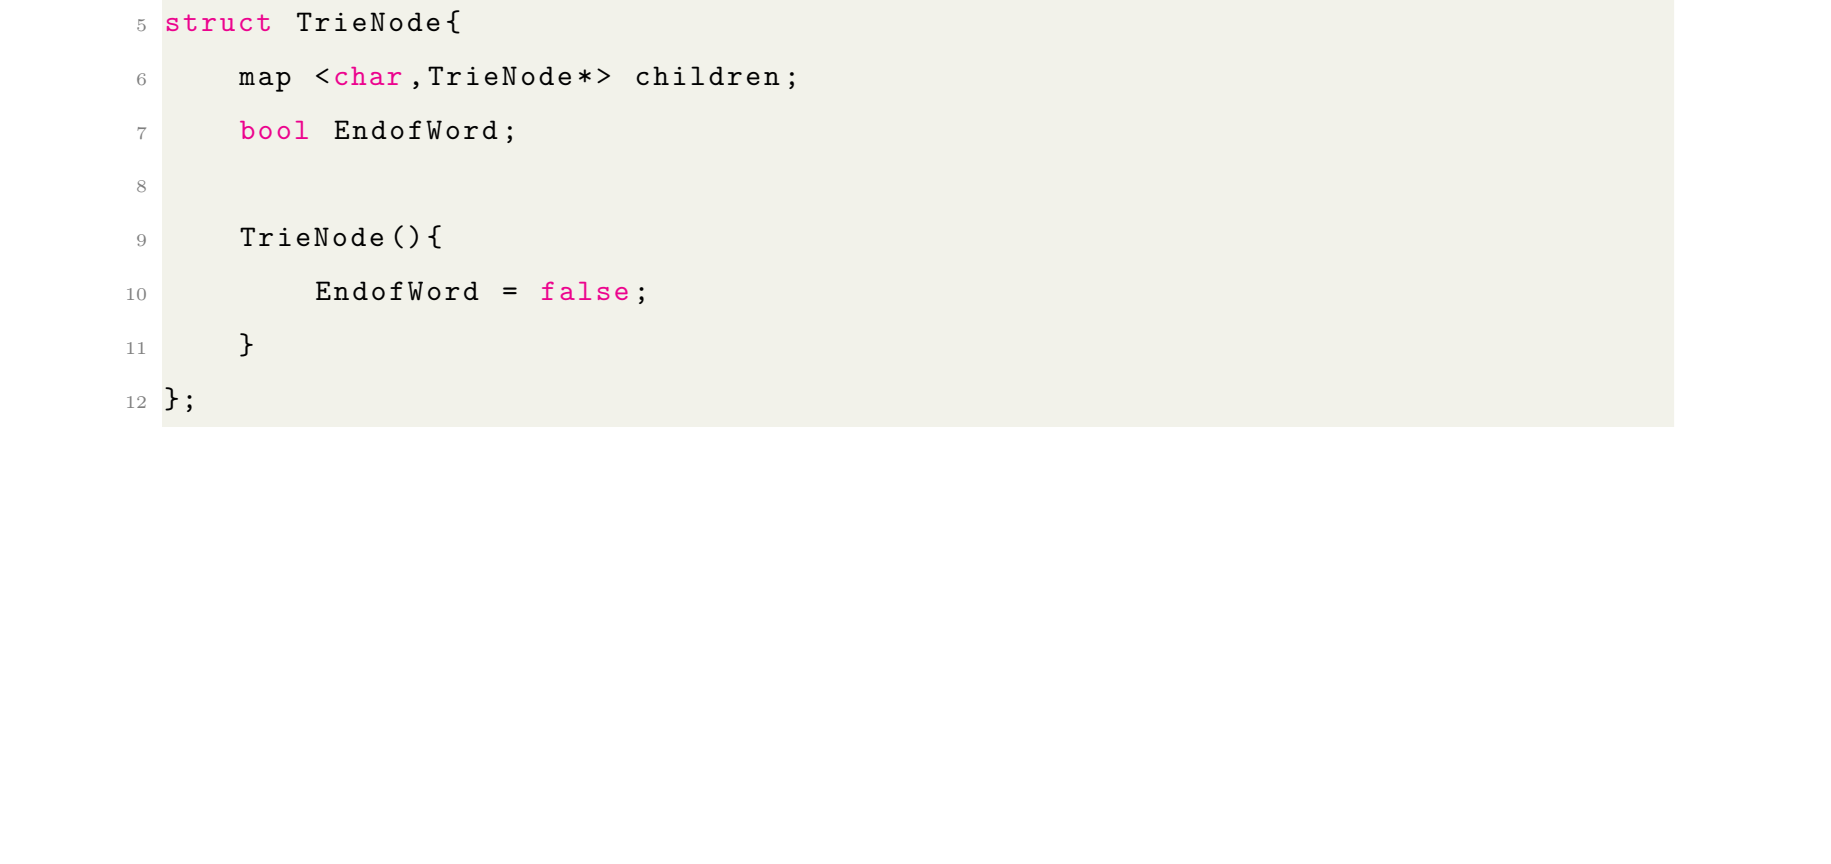
\includegraphics[scale=0.5]{se1.png}

\end{frame}

\begin{frame}{Insert: O(L)}
        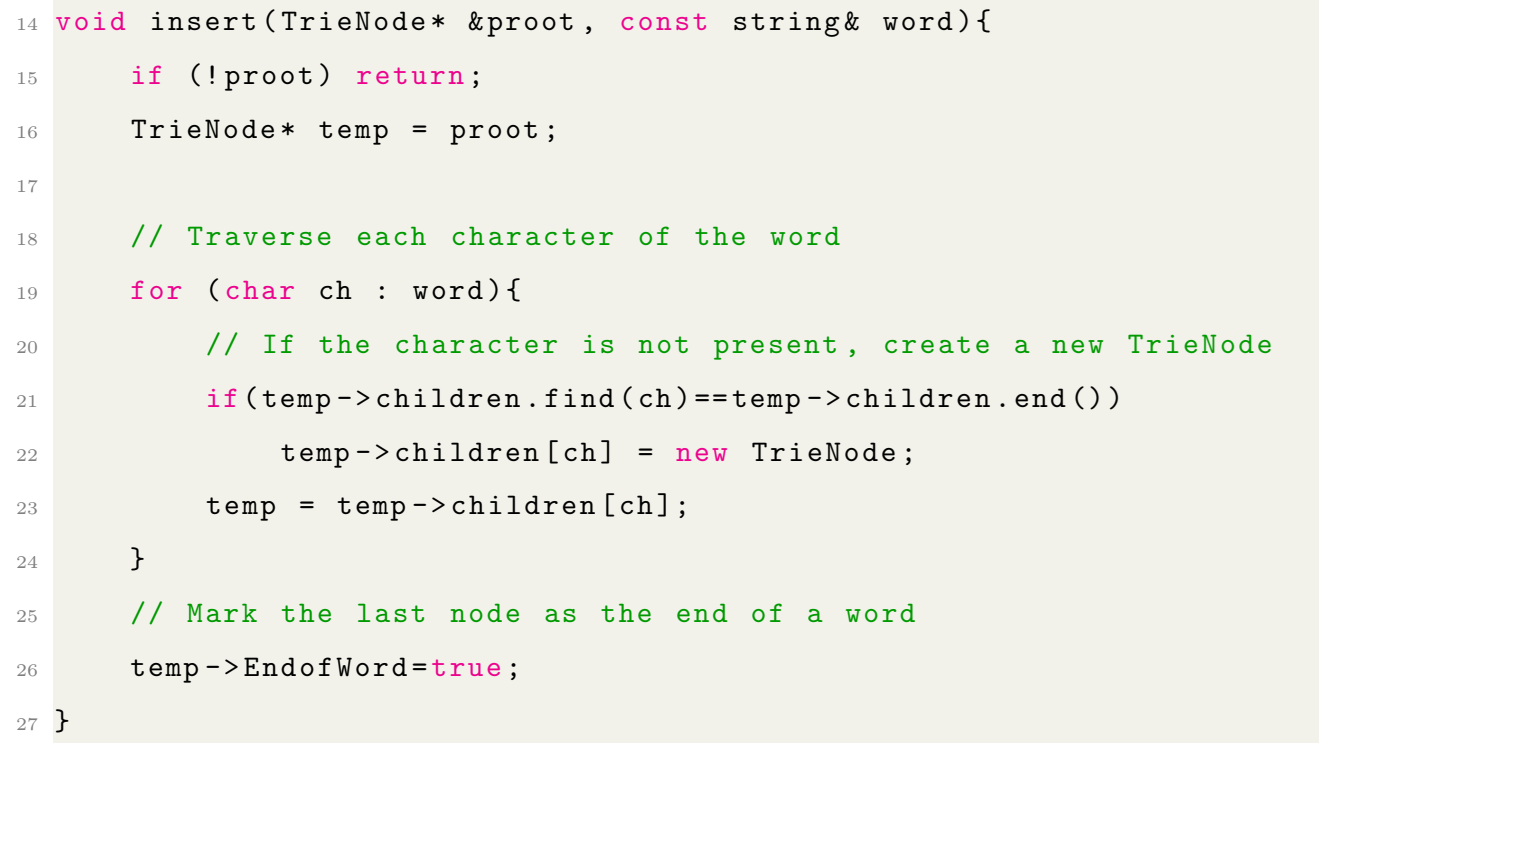
\includegraphics[scale=0.5]{se2.png}

\end{frame}
\begin{frame}{Visualize}
Assume we need to insert 5 words: 
\begin{itemize}[label=$\star$]
    \item app
    \item batman
    \item bat
    \item base
\end{itemize}
\end{frame}

\begin{frame}{Insert "apple"}
\begin{center}
      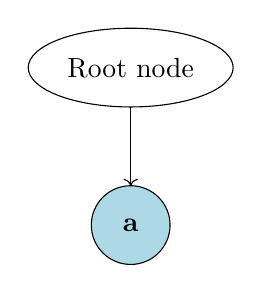
\begin{tikzpicture}
    \node[ellipse, draw, minimum width=2cm, minimum height=1cm] at (0,0) {Root node};
    \fill[blue] (0,-2) circle (0.5cm);
    \draw (0,-2) circle (0.5cm);
    \node at (0,-2) {\textbf{a}};
    \draw[->] (0,-0.5) -- (0,-1.5);
\end{tikzpicture}
\end{center}
  
\end{frame}
\begin{frame}{Insert "apple"}
    \begin{center}
        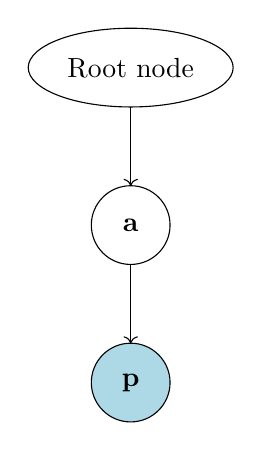
\begin{tikzpicture}
   \node[ellipse, draw, minimum width=2cm, minimum height=1cm] at (0,0) {Root node};
   
    \draw (0,-2) circle (0.5cm);
    \node at (0,-2) {\textbf{a}};
    \draw[->] (0,-0.5) -- (0,-1.5);
     \fill[blue] (0,-4) circle (0.5cm);
      \draw (0,-4) circle (0.5cm);
    \node at (0,-4) {\textbf{p}};
    \draw[->] (0,-2.5) -- (0,-3.5);
    
\end{tikzpicture}
    \end{center}
\end{frame}
\begin{frame}{Insert "apple"}
    \begin{center}
        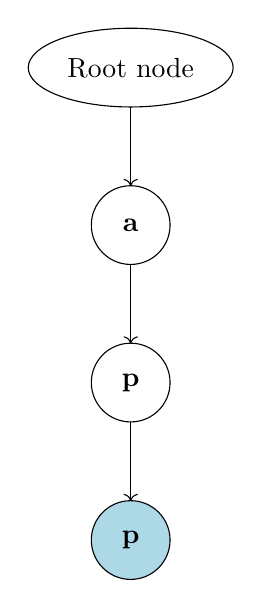
\begin{tikzpicture}
    % Hình elips "Root node"
    \node[ellipse, draw, minimum width=2cm, minimum height=1cm] at (0,0) {Root node};
    
    % Vòng tròn chứa "a" (không tô màu)
    \draw (0,-2) circle (0.5cm);
    \node at (0,-2) {\textbf{a}};
    \draw[->] (0,-0.5) -- (0,-1.5); % Mũi tên từ Root node tới "a"
    
    % Vòng tròn chứa "p" thứ nhất (không tô màu)
    \draw (0,-4) circle (0.5cm);
    \node at (0,-4) {\textbf{p}};
    \draw[->] (0,-2.5) -- (0,-3.5); % Mũi tên từ "a" tới "p"
    
    % Vòng tròn chứa "p" thứ hai (tô màu xanh dương)
    \fill[blue] (0,-6) circle (0.5cm); % Tô màu xanh dương
    \draw (0,-6) circle (0.5cm);
    \node at (0,-6) {\textbf{p}};
    \draw[->] (0,-4.5) -- (0,-5.5); % Mũi tên từ "p" trước tới "p" cuối
\end{tikzpicture}

    \end{center}
\end{frame}
\begin{frame}{Insert "apple"}
    \begin{center}
        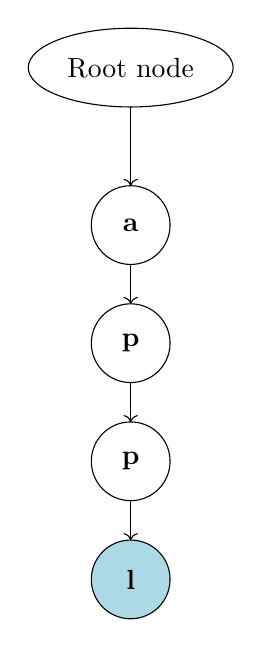
\begin{tikzpicture}
    % Hình elips "Root node"
    \node[ellipse, draw, minimum width=2cm, minimum height=1cm] at (0,0) {Root node};
    
    % Vòng tròn chứa "a" (không tô màu)
    \draw (0,-2) circle (0.5cm);
    \node at (0,-2) {\textbf{a}};
    \draw[->] (0,-0.5) -- (0,-1.5); % Mũi tên từ Root node tới "a"
    
    % Vòng tròn chứa "p" thứ nhất (không tô màu)
    \draw (0,-3.5) circle (0.5cm);
    \node at (0,-3.5) {\textbf{p}};
    \draw[->] (0,-2.5) -- (0,-3); % Mũi tên từ "a" tới "p"
    
    % Vòng tròn chứa "p" thứ hai (không tô màu)
    \draw (0,-5) circle (0.5cm);
    \node at (0,-5) {\textbf{p}};
    \draw[->] (0,-4) -- (0,-4.5); % Mũi tên từ "p" trước tới "p"
    
    % Vòng tròn chứa "l" (tô màu xanh dương)
    \fill[blue] (0,-6.5) circle (0.5cm); % Tô màu xanh dương
    \draw (0,-6.5) circle (0.5cm);
    \node at (0,-6.5) {\textbf{l}};
    \draw[->] (0,-5.5) -- (0,-6); % Mũi tên từ "p" tới "l"
\end{tikzpicture}
    \end{center}
\end{frame}
\begin{frame}{Insert "apple"}
\begin{center}
    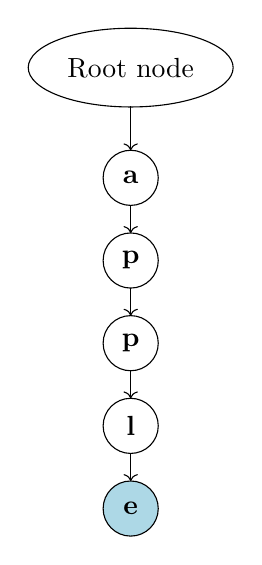
\begin{tikzpicture}[scale=0.7]
    % Vẽ hình elips chứa "Root node" tại tọa độ (0,0)
    \node[ellipse, draw, minimum width=2cm, minimum height=1cm] at (0,0) {Root node};
    
    % Vẽ vòng tròn chứa "a" tại (0,-2), không tô màu
    \draw (0,-2) circle (0.5cm);
    \node at (0,-2) {\textbf{a}}; % Chữ "a" in đậm ở tâm vòng tròn
    \draw[->] (0,-0.7) -- (0,-1.5); % Mũi tên từ dưới "Root node" tới trên "a"
    
    % Vẽ vòng tròn chứa "p" thứ nhất tại (0,-3.5), không tô màu
    \draw (0,-3.5) circle (0.5cm);
    \node at (0,-3.5) {\textbf{p}}; % Chữ "p" in đậm ở tâm vòng tròn
    \draw[->] (0,-2.5) -- (0,-3); % Mũi tên từ dưới "a" tới trên "p"
    
    % Vẽ vòng tròn chứa "p" thứ hai tại (0,-5), không tô màu
    \draw (0,-5) circle (0.5cm);
    \node at (0,-5) {\textbf{p}}; % Chữ "p" in đậm ở tâm vòng tròn
    \draw[->] (0,-4) -- (0,-4.5); % Mũi tên từ dưới "p" trước tới trên "p"
    
    % Vẽ vòng tròn chứa "l" tại (0,-6.5), không tô màu
    \draw (0,-6.5) circle (0.5cm);
    \node at (0,-6.5) {\textbf{l}}; % Chữ "l" in đậm ở tâm vòng tròn
    \draw[->] (0,-5.5) -- (0,-6); % Mũi tên từ dưới "p" tới trên "l"
    
    % Vẽ vòng tròn chứa "e" tại (0,-8), tô màu xanh dương
    \fill[blue] (0,-8) circle (0.5cm); % Tô nền màu xanh dương
    \draw (0,-8) circle (0.5cm); % Vẽ viền vòng tròn
    \node at (0,-8) {\textbf{e}}; % Chữ "e" in đậm ở tâm vòng tròn
    \draw[->] (0,-7) -- (0,-7.5); % Mũi tên từ dưới "l" tới trên "e"
\end{tikzpicture}
\end{center}
\end{frame}
\begin{frame}{Insert "apple"}
\begin{center}
    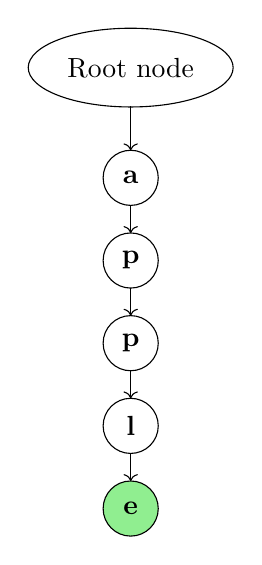
\begin{tikzpicture}[scale=0.7]
    % Vẽ hình elips chứa "Root node" tại tọa độ (0,0)
    \node[ellipse, draw, minimum width=2cm, minimum height=1cm] at (0,0) {Root node};
    
    % Vẽ vòng tròn chứa "a" tại (0,-2), không tô màu
    \draw (0,-2) circle (0.5cm);
    \node at (0,-2) {\textbf{a}}; % Chữ "a" in đậm ở tâm vòng tròn
    \draw[->] (0,-0.7) -- (0,-1.5); % Mũi tên từ dưới "Root node" tới trên "a"
    
    % Vẽ vòng tròn chứa "p" thứ nhất tại (0,-3.5), không tô màu
    \draw (0,-3.5) circle (0.5cm);
    \node at (0,-3.5) {\textbf{p}}; % Chữ "p" in đậm ở tâm vòng tròn
    \draw[->] (0,-2.5) -- (0,-3); % Mũi tên từ dưới "a" tới trên "p"
    
    % Vẽ vòng tròn chứa "p" thứ hai tại (0,-5), không tô màu
    \draw (0,-5) circle (0.5cm);
    \node at (0,-5) {\textbf{p}}; % Chữ "p" in đậm ở tâm vòng tròn
    \draw[->] (0,-4) -- (0,-4.5); % Mũi tên từ dưới "p" trước tới trên "p"
    
    % Vẽ vòng tròn chứa "l" tại (0,-6.5), không tô màu
    \draw (0,-6.5) circle (0.5cm);
    \node at (0,-6.5) {\textbf{l}}; % Chữ "l" in đậm ở tâm vòng tròn
    \draw[->] (0,-5.5) -- (0,-6); % Mũi tên từ dưới "p" tới trên "l"
    
    % Vẽ vòng tròn chứa "e" tại (0,-8), tô màu xanh dương
    \fill[green] (0,-8) circle (0.5cm); % Tô nền màu xanh dương
    \draw (0,-8) circle (0.5cm); % Vẽ viền vòng tròn
    \node at (0,-8) {\textbf{e}}; % Chữ "e" in đậm ở tâm vòng tròn
    \draw[->] (0,-7) -- (0,-7.5); % Mũi tên từ dưới "l" tới trên "e"
\end{tikzpicture}
\end{center}
\end{frame}
\begin{frame}{Insert "app"}
\begin{center}
    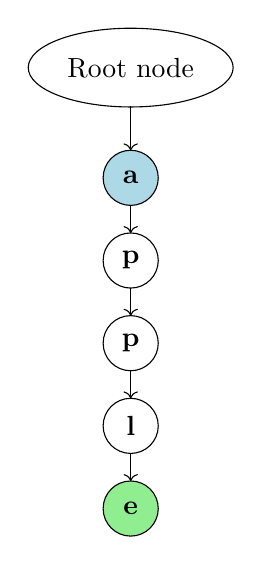
\begin{tikzpicture}[scale=0.7]
    % Vẽ hình elips chứa "Root node" tại tọa độ (0,0)
    \node[ellipse, draw, minimum width=2cm, minimum height=1cm] at (0,0) {Root node};
    
    % Vẽ vòng tròn chứa "a" tại (0,-2), không tô màu
     \fill[blue] (0,-2) circle (0.5cm);
    \draw (0,-2) circle (0.5cm);
    \node at (0,-2) {\textbf{a}}; % Chữ "a" in đậm ở tâm vòng tròn
    \draw[->] (0,-0.7) -- (0,-1.5); % Mũi tên từ dưới "Root node" tới trên "a"
    
    % Vẽ vòng tròn chứa "p" thứ nhất tại (0,-3.5), không tô màu
    \draw (0,-3.5) circle (0.5cm);
    \node at (0,-3.5) {\textbf{p}}; % Chữ "p" in đậm ở tâm vòng tròn
    \draw[->] (0,-2.5) -- (0,-3); % Mũi tên từ dưới "a" tới trên "p"
    
    % Vẽ vòng tròn chứa "p" thứ hai tại (0,-5), không tô màu
    \draw (0,-5) circle (0.5cm);
    \node at (0,-5) {\textbf{p}}; % Chữ "p" in đậm ở tâm vòng tròn
    \draw[->] (0,-4) -- (0,-4.5); % Mũi tên từ dưới "p" trước tới trên "p"
    
    % Vẽ vòng tròn chứa "l" tại (0,-6.5), không tô màu
    \draw (0,-6.5) circle (0.5cm);
    \node at (0,-6.5) {\textbf{l}}; % Chữ "l" in đậm ở tâm vòng tròn
    \draw[->] (0,-5.5) -- (0,-6); % Mũi tên từ dưới "p" tới trên "l"
    
    % Vẽ vòng tròn chứa "e" tại (0,-8), tô màu xanh dương
    \fill[green] (0,-8) circle (0.5cm); % Tô nền màu xanh dương
    \draw (0,-8) circle (0.5cm); % Vẽ viền vòng tròn
    \node at (0,-8) {\textbf{e}}; % Chữ "e" in đậm ở tâm vòng tròn
    \draw[->] (0,-7) -- (0,-7.5); % Mũi tên từ dưới "l" tới trên "e"
\end{tikzpicture}
\end{center}
\end{frame}
\begin{frame}{Insert "app"}
\begin{center}
    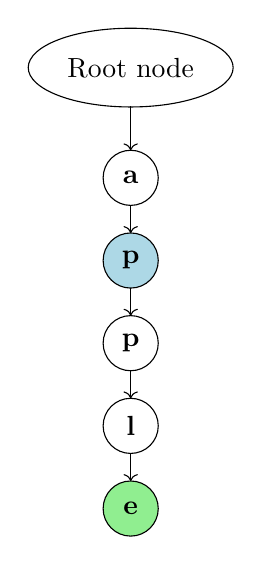
\begin{tikzpicture}[scale=0.7]
    % Vẽ hình elips chứa "Root node" tại tọa độ (0,0)
    \node[ellipse, draw, minimum width=2cm, minimum height=1cm] at (0,0) {Root node};
    
    % Vẽ vòng tròn chứa "a" tại (0,-2), không tô màu
     \fill[blue] (0,-3.5) circle (0.5cm);
    \draw (0,-2) circle (0.5cm);
    \node at (0,-2) {\textbf{a}}; % Chữ "a" in đậm ở tâm vòng tròn
    \draw[->] (0,-0.7) -- (0,-1.5); % Mũi tên từ dưới "Root node" tới trên "a"
    
    % Vẽ vòng tròn chứa "p" thứ nhất tại (0,-3.5), không tô màu
    \draw (0,-3.5) circle (0.5cm);
    \node at (0,-3.5) {\textbf{p}}; % Chữ "p" in đậm ở tâm vòng tròn
    \draw[->] (0,-2.5) -- (0,-3); % Mũi tên từ dưới "a" tới trên "p"
    
    % Vẽ vòng tròn chứa "p" thứ hai tại (0,-5), không tô màu
    \draw (0,-5) circle (0.5cm);
    \node at (0,-5) {\textbf{p}}; % Chữ "p" in đậm ở tâm vòng tròn
    \draw[->] (0,-4) -- (0,-4.5); % Mũi tên từ dưới "p" trước tới trên "p"
    
    % Vẽ vòng tròn chứa "l" tại (0,-6.5), không tô màu
    \draw (0,-6.5) circle (0.5cm);
    \node at (0,-6.5) {\textbf{l}}; % Chữ "l" in đậm ở tâm vòng tròn
    \draw[->] (0,-5.5) -- (0,-6); % Mũi tên từ dưới "p" tới trên "l"
    
    % Vẽ vòng tròn chứa "e" tại (0,-8), tô màu xanh dương
    \fill[green] (0,-8) circle (0.5cm); % Tô nền màu xanh dương
    \draw (0,-8) circle (0.5cm); % Vẽ viền vòng tròn
    \node at (0,-8) {\textbf{e}}; % Chữ "e" in đậm ở tâm vòng tròn
    \draw[->] (0,-7) -- (0,-7.5); % Mũi tên từ dưới "l" tới trên "e"
\end{tikzpicture}

\end{center}
\end{frame}
\begin{frame}{Insert "app"}
\begin{center}
    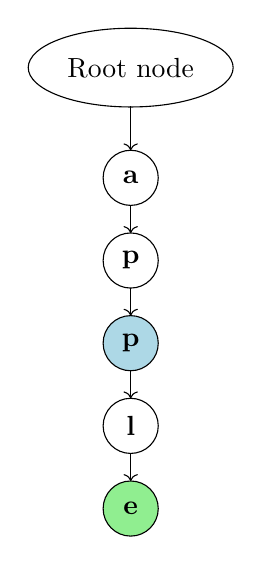
\begin{tikzpicture}[scale=0.7]
    % Vẽ hình elips chứa "Root node" tại tọa độ (0,0)
    \node[ellipse, draw, minimum width=2cm, minimum height=1cm] at (0,0) {Root node};
    
    % Vẽ vòng tròn chứa "a" tại (0,-2), không tô màu
     \fill[blue] (0,-5) circle (0.5cm);
    \draw (0,-2) circle (0.5cm);
    \node at (0,-2) {\textbf{a}}; % Chữ "a" in đậm ở tâm vòng tròn
    \draw[->] (0,-0.7) -- (0,-1.5); % Mũi tên từ dưới "Root node" tới trên "a"
    
    % Vẽ vòng tròn chứa "p" thứ nhất tại (0,-3.5), không tô màu
    \draw (0,-3.5) circle (0.5cm);
    \node at (0,-3.5) {\textbf{p}}; % Chữ "p" in đậm ở tâm vòng tròn
    \draw[->] (0,-2.5) -- (0,-3); % Mũi tên từ dưới "a" tới trên "p"
    
    % Vẽ vòng tròn chứa "p" thứ hai tại (0,-5), không tô màu
    \draw (0,-5) circle (0.5cm);
    \node at (0,-5) {\textbf{p}}; % Chữ "p" in đậm ở tâm vòng tròn
    \draw[->] (0,-4) -- (0,-4.5); % Mũi tên từ dưới "p" trước tới trên "p"
    
    % Vẽ vòng tròn chứa "l" tại (0,-6.5), không tô màu
    \draw (0,-6.5) circle (0.5cm);
    \node at (0,-6.5) {\textbf{l}}; % Chữ "l" in đậm ở tâm vòng tròn
    \draw[->] (0,-5.5) -- (0,-6); % Mũi tên từ dưới "p" tới trên "l"
    
    % Vẽ vòng tròn chứa "e" tại (0,-8), tô màu xanh dương
    \fill[green] (0,-8) circle (0.5cm); % Tô nền màu xanh dương
    \draw (0,-8) circle (0.5cm); % Vẽ viền vòng tròn
    \node at (0,-8) {\textbf{e}}; % Chữ "e" in đậm ở tâm vòng tròn
    \draw[->] (0,-7) -- (0,-7.5); % Mũi tên từ dưới "l" tới trên "e"
\end{tikzpicture}

\end{center}
\end{frame}
\begin{frame}{Insert "app"}
\begin{center}
    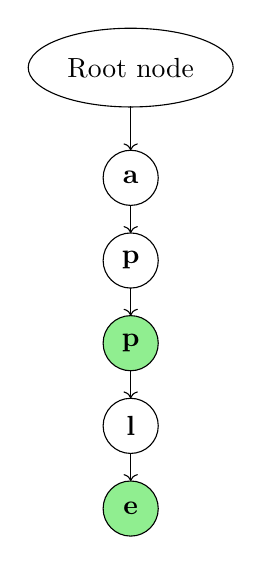
\begin{tikzpicture}[scale=0.7]
    % Vẽ hình elips chứa "Root node" tại tọa độ (0,0)
    \node[ellipse, draw, minimum width=2cm, minimum height=1cm] at (0,0) {Root node};
    
    % Vẽ vòng tròn chứa "a" tại (0,-2), không tô màu
     \fill[green] (0,-5) circle (0.5cm);
    \draw (0,-2) circle (0.5cm);
    \node at (0,-2) {\textbf{a}}; % Chữ "a" in đậm ở tâm vòng tròn
    \draw[->] (0,-0.7) -- (0,-1.5); % Mũi tên từ dưới "Root node" tới trên "a"
    
    % Vẽ vòng tròn chứa "p" thứ nhất tại (0,-3.5), không tô màu
    \draw (0,-3.5) circle (0.5cm);
    \node at (0,-3.5) {\textbf{p}}; % Chữ "p" in đậm ở tâm vòng tròn
    \draw[->] (0,-2.5) -- (0,-3); % Mũi tên từ dưới "a" tới trên "p"
    
    % Vẽ vòng tròn chứa "p" thứ hai tại (0,-5), không tô màu
    \draw (0,-5) circle (0.5cm);
    \node at (0,-5) {\textbf{p}}; % Chữ "p" in đậm ở tâm vòng tròn
    \draw[->] (0,-4) -- (0,-4.5); % Mũi tên từ dưới "p" trước tới trên "p"
    
    % Vẽ vòng tròn chứa "l" tại (0,-6.5), không tô màu
    \draw (0,-6.5) circle (0.5cm);
    \node at (0,-6.5) {\textbf{l}}; % Chữ "l" in đậm ở tâm vòng tròn
    \draw[->] (0,-5.5) -- (0,-6); % Mũi tên từ dưới "p" tới trên "l"
    
    % Vẽ vòng tròn chứa "e" tại (0,-8), tô màu xanh dương
    \fill[green] (0,-8) circle (0.5cm); % Tô nền màu xanh dương
    \draw (0,-8) circle (0.5cm); % Vẽ viền vòng tròn
    \node at (0,-8) {\textbf{e}}; % Chữ "e" in đậm ở tâm vòng tròn
    \draw[->] (0,-7) -- (0,-7.5); % Mũi tên từ dưới "l" tới trên "e"
\end{tikzpicture}
\end{center}
\end{frame}
\begin{frame}{Insert "bat"}
\begin{center}
    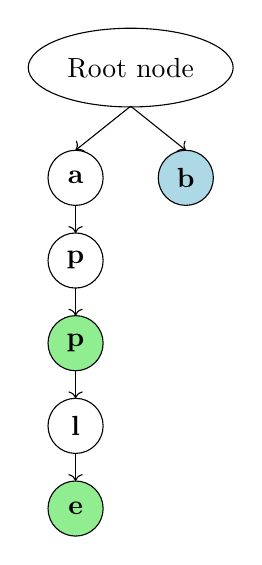
\begin{tikzpicture}[scale=0.7]
    % Vẽ hình elips chứa "Root node" tại tọa độ (0,0)
    \node[ellipse, draw, minimum width=2cm, minimum height=1cm] at (1,0) {Root node};
    
    % Vẽ vòng tròn chứa "a" tại (0,-2), không tô màu
     \fill[green] (0,-5) circle (0.5cm);
    \draw (0,-2) circle (0.5cm);
    \node at (0,-2) {\textbf{a}}; % Chữ "a" in đậm ở tâm vòng tròn
    \draw[->] (1,-0.7) -- (0,-1.5); % Mũi tên từ dưới "Root node" tới trên "a"
    
    % Vẽ vòng tròn chứa "p" thứ nhất tại (0,-3.5), không tô màu
    \draw (0,-3.5) circle (0.5cm);
    \node at (0,-3.5) {\textbf{p}}; % Chữ "p" in đậm ở tâm vòng tròn
    \draw[->] (0,-2.5) -- (0,-3); % Mũi tên từ dưới "a" tới trên "p"
    
    % Vẽ vòng tròn chứa "p" thứ hai tại (0,-5), không tô màu
    \draw (0,-5) circle (0.5cm);
    \node at (0,-5) {\textbf{p}}; % Chữ "p" in đậm ở tâm vòng tròn
    \draw[->] (0,-4) -- (0,-4.5); % Mũi tên từ dưới "p" trước tới trên "p"
    
    % Vẽ vòng tròn chứa "l" tại (0,-6.5), không tô màu
    \draw (0,-6.5) circle (0.5cm);
    \node at (0,-6.5) {\textbf{l}}; % Chữ "l" in đậm ở tâm vòng tròn
    \draw[->] (0,-5.5) -- (0,-6); % Mũi tên từ dưới "p" tới trên "l"
    
    % Vẽ vòng tròn chứa "e" tại (0,-8), tô màu xanh dương
    \fill[green] (0,-8) circle (0.5cm); % Tô nền màu xanh dương
    \draw (0,-8) circle (0.5cm); % Vẽ viền vòng tròn
    \node at (0,-8) {\textbf{e}}; % Chữ "e" in đậm ở tâm vòng tròn
    \draw[->] (0,-7) -- (0,-7.5); % Mũi tên từ dưới "l" tới trên "e"

    %b
    \fill[blue] (2,-2) circle (0.5cm);
    \draw (2,-2) circle (0.5cm);
    \node at (2,-2) {\textbf{b}}; % Chữ "a" in đậm ở tâm vòng tròn
    \draw[->] (1,-0.7) -- (2,-1.5); % Mũi tên từ dưới "Root node" tới trên "a"
    
\end{tikzpicture}
\end{center}
\end{frame}
\begin{frame}{Insert "bat"}
\begin{center}
    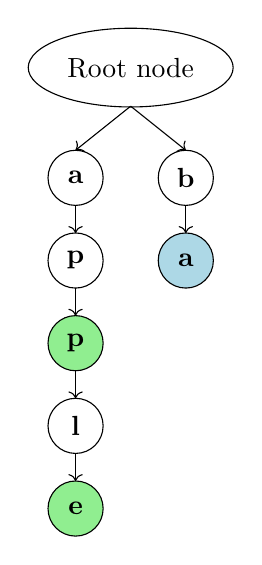
\begin{tikzpicture}[scale=0.7]
    % Vẽ hình elips chứa "Root node" tại tọa độ (0,0)
    \node[ellipse, draw, minimum width=2cm, minimum height=1cm] at (1,0) {Root node};
    
    % Vẽ vòng tròn chứa "a" tại (0,-2), không tô màu
     \fill[green] (0,-5) circle (0.5cm);
    \draw (0,-2) circle (0.5cm);
    \node at (0,-2) {\textbf{a}}; % Chữ "a" in đậm ở tâm vòng tròn
    \draw[->] (1,-0.7) -- (0,-1.5); % Mũi tên từ dưới "Root node" tới trên "a"
    
    % Vẽ vòng tròn chứa "p" thứ nhất tại (0,-3.5), không tô màu
    \draw (0,-3.5) circle (0.5cm);
    \node at (0,-3.5) {\textbf{p}}; % Chữ "p" in đậm ở tâm vòng tròn
    \draw[->] (0,-2.5) -- (0,-3); % Mũi tên từ dưới "a" tới trên "p"
    
    % Vẽ vòng tròn chứa "p" thứ hai tại (0,-5), không tô màu
    \draw (0,-5) circle (0.5cm);
    \node at (0,-5) {\textbf{p}}; % Chữ "p" in đậm ở tâm vòng tròn
    \draw[->] (0,-4) -- (0,-4.5); % Mũi tên từ dưới "p" trước tới trên "p"
    
    % Vẽ vòng tròn chứa "l" tại (0,-6.5), không tô màu
    \draw (0,-6.5) circle (0.5cm);
    \node at (0,-6.5) {\textbf{l}}; % Chữ "l" in đậm ở tâm vòng tròn
    \draw[->] (0,-5.5) -- (0,-6); % Mũi tên từ dưới "p" tới trên "l"
    
    % Vẽ vòng tròn chứa "e" tại (0,-8), tô màu xanh dương
    \fill[green] (0,-8) circle (0.5cm); % Tô nền màu xanh dương
    \draw (0,-8) circle (0.5cm); % Vẽ viền vòng tròn
    \node at (0,-8) {\textbf{e}}; % Chữ "e" in đậm ở tâm vòng tròn
    \draw[->] (0,-7) -- (0,-7.5); % Mũi tên từ dưới "l" tới trên "e"

    %b
    \draw (2,-2) circle (0.5cm);
    \node at (2,-2) {\textbf{b}}; % Chữ "a" in đậm ở tâm vòng tròn
    \draw[->] (1,-0.7) -- (2,-1.5); % Mũi tên từ dưới "Root node" tới trên "a"
    %a
    \fill[blue] (2,-3.5) circle (0.5cm);
    \draw (2,-3.5) circle (0.5cm);
    \node at (2,-3.5) {\textbf{a}}; % Chữ "a" in đậm ở tâm vòng tròn
    \draw[->] (2,-2.5) -- (2,-3); % Mũi tên từ dưới "Root node" tới trên "a"
    
\end{tikzpicture}
\end{center}
\end{frame}
\begin{frame}{Insert "bat"}
\begin{center}
    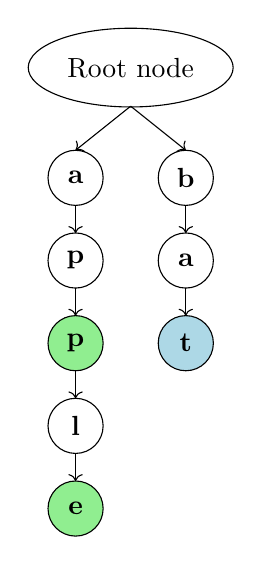
\begin{tikzpicture}[scale=0.7]
    % Vẽ hình elips chứa "Root node" tại tọa độ (0,0)
    \node[ellipse, draw, minimum width=2cm, minimum height=1cm] at (1,0) {Root node};
    
    % Vẽ vòng tròn chứa "a" tại (0,-2), không tô màu
     \fill[green] (0,-5) circle (0.5cm);
    \draw (0,-2) circle (0.5cm);
    \node at (0,-2) {\textbf{a}}; % Chữ "a" in đậm ở tâm vòng tròn
    \draw[->] (1,-0.7) -- (0,-1.5); % Mũi tên từ dưới "Root node" tới trên "a"
    
    % Vẽ vòng tròn chứa "p" thứ nhất tại (0,-3.5), không tô màu
    \draw (0,-3.5) circle (0.5cm);
    \node at (0,-3.5) {\textbf{p}}; % Chữ "p" in đậm ở tâm vòng tròn
    \draw[->] (0,-2.5) -- (0,-3); % Mũi tên từ dưới "a" tới trên "p"
    
    % Vẽ vòng tròn chứa "p" thứ hai tại (0,-5), không tô màu
    \draw (0,-5) circle (0.5cm);
    \node at (0,-5) {\textbf{p}}; % Chữ "p" in đậm ở tâm vòng tròn
    \draw[->] (0,-4) -- (0,-4.5); % Mũi tên từ dưới "p" trước tới trên "p"
    
    % Vẽ vòng tròn chứa "l" tại (0,-6.5), không tô màu
    \draw (0,-6.5) circle (0.5cm);
    \node at (0,-6.5) {\textbf{l}}; % Chữ "l" in đậm ở tâm vòng tròn
    \draw[->] (0,-5.5) -- (0,-6); % Mũi tên từ dưới "p" tới trên "l"
    
    % Vẽ vòng tròn chứa "e" tại (0,-8), tô màu xanh dương
    \fill[green] (0,-8) circle (0.5cm); % Tô nền màu xanh dương
    \draw (0,-8) circle (0.5cm); % Vẽ viền vòng tròn
    \node at (0,-8) {\textbf{e}}; % Chữ "e" in đậm ở tâm vòng tròn
    \draw[->] (0,-7) -- (0,-7.5); % Mũi tên từ dưới "l" tới trên "e"

    %b
    \draw (2,-2) circle (0.5cm);
    \node at (2,-2) {\textbf{b}}; % Chữ "a" in đậm ở tâm vòng tròn
    \draw[->] (1,-0.7) -- (2,-1.5); % Mũi tên từ dưới "Root node" tới trên "a"
    %a
    \draw (2,-3.5) circle (0.5cm);
    \node at (2,-3.5) {\textbf{a}}; % Chữ "a" in đậm ở tâm vòng tròn
    \draw[->] (2,-2.5) -- (2,-3); % Mũi tên từ dưới "Root node" tới trên "a"
    %t
    \fill[blue] (2,-5) circle (0.5cm);
    \draw (2,-5) circle (0.5cm);
    \node at (2,-5) {\textbf{t}}; % Chữ "p" in đậm ở tâm vòng tròn
    \draw[->] (2,-4) -- (2,-4.5); % Mũi tên từ dưới "p" trước tới trên "p"
    
    
\end{tikzpicture}
\end{center}
\end{frame}
\begin{frame}{Insert "bat"}
\begin{center}
    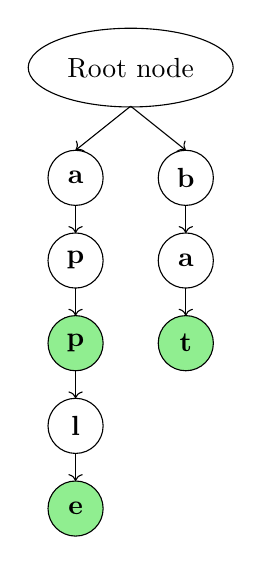
\begin{tikzpicture}[scale=0.7]
    % Vẽ hình elips chứa "Root node" tại tọa độ (0,0)
    \node[ellipse, draw, minimum width=2cm, minimum height=1cm] at (1,0) {Root node};
    
    % Vẽ vòng tròn chứa "a" tại (0,-2), không tô màu
     \fill[green] (0,-5) circle (0.5cm);
    \draw (0,-2) circle (0.5cm);
    \node at (0,-2) {\textbf{a}}; % Chữ "a" in đậm ở tâm vòng tròn
    \draw[->] (1,-0.7) -- (0,-1.5); % Mũi tên từ dưới "Root node" tới trên "a"
    
    % Vẽ vòng tròn chứa "p" thứ nhất tại (0,-3.5), không tô màu
    \draw (0,-3.5) circle (0.5cm);
    \node at (0,-3.5) {\textbf{p}}; % Chữ "p" in đậm ở tâm vòng tròn
    \draw[->] (0,-2.5) -- (0,-3); % Mũi tên từ dưới "a" tới trên "p"
    
    % Vẽ vòng tròn chứa "p" thứ hai tại (0,-5), không tô màu
    \draw (0,-5) circle (0.5cm);
    \node at (0,-5) {\textbf{p}}; % Chữ "p" in đậm ở tâm vòng tròn
    \draw[->] (0,-4) -- (0,-4.5); % Mũi tên từ dưới "p" trước tới trên "p"
    
    % Vẽ vòng tròn chứa "l" tại (0,-6.5), không tô màu
    \draw (0,-6.5) circle (0.5cm);
    \node at (0,-6.5) {\textbf{l}}; % Chữ "l" in đậm ở tâm vòng tròn
    \draw[->] (0,-5.5) -- (0,-6); % Mũi tên từ dưới "p" tới trên "l"
    
    % Vẽ vòng tròn chứa "e" tại (0,-8), tô màu xanh dương
    \fill[green] (0,-8) circle (0.5cm); % Tô nền màu xanh dương
    \draw (0,-8) circle (0.5cm); % Vẽ viền vòng tròn
    \node at (0,-8) {\textbf{e}}; % Chữ "e" in đậm ở tâm vòng tròn
    \draw[->] (0,-7) -- (0,-7.5); % Mũi tên từ dưới "l" tới trên "e"

    %b
    \draw (2,-2) circle (0.5cm);
    \node at (2,-2) {\textbf{b}}; % Chữ "a" in đậm ở tâm vòng tròn
    \draw[->] (1,-0.7) -- (2,-1.5); % Mũi tên từ dưới "Root node" tới trên "a"
    %a
    \draw (2,-3.5) circle (0.5cm);
    \node at (2,-3.5) {\textbf{a}}; % Chữ "a" in đậm ở tâm vòng tròn
    \draw[->] (2,-2.5) -- (2,-3); % Mũi tên từ dưới "Root node" tới trên "a"
    %t
    \fill[green] (2,-5) circle (0.5cm);
    \draw (2,-5) circle (0.5cm);
    \node at (2,-5) {\textbf{t}}; % Chữ "p" in đậm ở tâm vòng tròn
    \draw[->] (2,-4) -- (2,-4.5); % Mũi tên từ dưới "p" trước tới trên "p"
    
    
\end{tikzpicture}
\end{center}
\end{frame}
\begin{frame}{Insert "batman"}
\begin{center}
    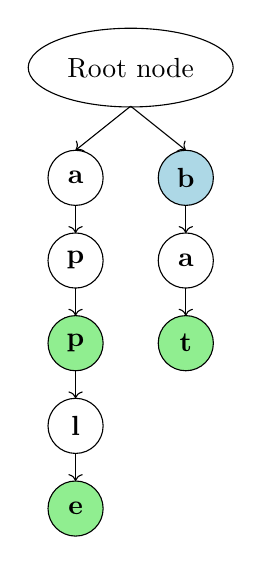
\begin{tikzpicture}[scale=0.7]
    % Vẽ hình elips chứa "Root node" tại tọa độ (0,0)
    \node[ellipse, draw, minimum width=2cm, minimum height=1cm] at (1,0) {Root node};
    
    % Vẽ vòng tròn chứa "a" tại (0,-2), không tô màu
     \fill[green] (0,-5) circle (0.5cm);
    \draw (0,-2) circle (0.5cm);
    \node at (0,-2) {\textbf{a}}; % Chữ "a" in đậm ở tâm vòng tròn
    \draw[->] (1,-0.7) -- (0,-1.5); % Mũi tên từ dưới "Root node" tới trên "a"
    
    % Vẽ vòng tròn chứa "p" thứ nhất tại (0,-3.5), không tô màu
    \draw (0,-3.5) circle (0.5cm);
    \node at (0,-3.5) {\textbf{p}}; % Chữ "p" in đậm ở tâm vòng tròn
    \draw[->] (0,-2.5) -- (0,-3); % Mũi tên từ dưới "a" tới trên "p"
    
    % Vẽ vòng tròn chứa "p" thứ hai tại (0,-5), không tô màu
    \draw (0,-5) circle (0.5cm);
    \node at (0,-5) {\textbf{p}}; % Chữ "p" in đậm ở tâm vòng tròn
    \draw[->] (0,-4) -- (0,-4.5); % Mũi tên từ dưới "p" trước tới trên "p"
    
    % Vẽ vòng tròn chứa "l" tại (0,-6.5), không tô màu
    \draw (0,-6.5) circle (0.5cm);
    \node at (0,-6.5) {\textbf{l}}; % Chữ "l" in đậm ở tâm vòng tròn
    \draw[->] (0,-5.5) -- (0,-6); % Mũi tên từ dưới "p" tới trên "l"
    
    % Vẽ vòng tròn chứa "e" tại (0,-8), tô màu xanh dương
    \fill[green] (0,-8) circle (0.5cm); % Tô nền màu xanh dương
    \draw (0,-8) circle (0.5cm); % Vẽ viền vòng tròn
    \node at (0,-8) {\textbf{e}}; % Chữ "e" in đậm ở tâm vòng tròn
    \draw[->] (0,-7) -- (0,-7.5); % Mũi tên từ dưới "l" tới trên "e"

    %b
     \fill[blue] (2,-2) circle (0.5cm);
    \draw (2,-2) circle (0.5cm);
    \node at (2,-2) {\textbf{b}}; % Chữ "a" in đậm ở tâm vòng tròn
    \draw[->] (1,-0.7) -- (2,-1.5); % Mũi tên từ dưới "Root node" tới trên "a"
    %a
    \draw (2,-3.5) circle (0.5cm);
    \node at (2,-3.5) {\textbf{a}}; % Chữ "a" in đậm ở tâm vòng tròn
    \draw[->] (2,-2.5) -- (2,-3); % Mũi tên từ dưới "Root node" tới trên "a"
    %t
    \fill[green] (2,-5) circle (0.5cm);
    \draw (2,-5) circle (0.5cm);
    \node at (2,-5) {\textbf{t}}; % Chữ "p" in đậm ở tâm vòng tròn
    \draw[->] (2,-4) -- (2,-4.5); % Mũi tên từ dưới "p" trước tới trên "p"
    
    
\end{tikzpicture}

\end{center}
\end{frame}
\begin{frame}{Insert "batman"}
\begin{center}
    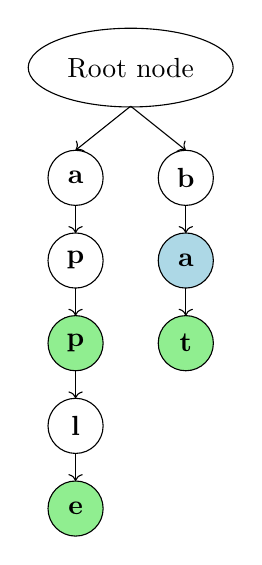
\begin{tikzpicture}[scale=0.7]
    % Vẽ hình elips chứa "Root node" tại tọa độ (0,0)
    \node[ellipse, draw, minimum width=2cm, minimum height=1cm] at (1,0) {Root node};
    
    % Vẽ vòng tròn chứa "a" tại (0,-2), không tô màu
     \fill[green] (0,-5) circle (0.5cm);
    \draw (0,-2) circle (0.5cm);
    \node at (0,-2) {\textbf{a}}; % Chữ "a" in đậm ở tâm vòng tròn
    \draw[->] (1,-0.7) -- (0,-1.5); % Mũi tên từ dưới "Root node" tới trên "a"
    
    % Vẽ vòng tròn chứa "p" thứ nhất tại (0,-3.5), không tô màu
    \draw (0,-3.5) circle (0.5cm);
    \node at (0,-3.5) {\textbf{p}}; % Chữ "p" in đậm ở tâm vòng tròn
    \draw[->] (0,-2.5) -- (0,-3); % Mũi tên từ dưới "a" tới trên "p"
    
    % Vẽ vòng tròn chứa "p" thứ hai tại (0,-5), không tô màu
    \draw (0,-5) circle (0.5cm);
    \node at (0,-5) {\textbf{p}}; % Chữ "p" in đậm ở tâm vòng tròn
    \draw[->] (0,-4) -- (0,-4.5); % Mũi tên từ dưới "p" trước tới trên "p"
    
    % Vẽ vòng tròn chứa "l" tại (0,-6.5), không tô màu
    \draw (0,-6.5) circle (0.5cm);
    \node at (0,-6.5) {\textbf{l}}; % Chữ "l" in đậm ở tâm vòng tròn
    \draw[->] (0,-5.5) -- (0,-6); % Mũi tên từ dưới "p" tới trên "l"
    
    % Vẽ vòng tròn chứa "e" tại (0,-8), tô màu xanh dương
    \fill[green] (0,-8) circle (0.5cm); % Tô nền màu xanh dương
    \draw (0,-8) circle (0.5cm); % Vẽ viền vòng tròn
    \node at (0,-8) {\textbf{e}}; % Chữ "e" in đậm ở tâm vòng tròn
    \draw[->] (0,-7) -- (0,-7.5); % Mũi tên từ dưới "l" tới trên "e"

    %b
     \fill[blue] (2,-3.5) circle (0.5cm);
    \draw (2,-2) circle (0.5cm);
    \node at (2,-2) {\textbf{b}}; % Chữ "a" in đậm ở tâm vòng tròn
    \draw[->] (1,-0.7) -- (2,-1.5); % Mũi tên từ dưới "Root node" tới trên "a"
    %a
    \draw (2,-3.5) circle (0.5cm);
    \node at (2,-3.5) {\textbf{a}}; % Chữ "a" in đậm ở tâm vòng tròn
    \draw[->] (2,-2.5) -- (2,-3); % Mũi tên từ dưới "Root node" tới trên "a"
    %t
    \fill[green] (2,-5) circle (0.5cm);
    \draw (2,-5) circle (0.5cm);
    \node at (2,-5) {\textbf{t}}; % Chữ "p" in đậm ở tâm vòng tròn
    \draw[->] (2,-4) -- (2,-4.5); % Mũi tên từ dưới "p" trước tới trên "p"
    
    
\end{tikzpicture}
\end{center}
\end{frame}
\begin{frame}{Insert "batman"}
\begin{center}
    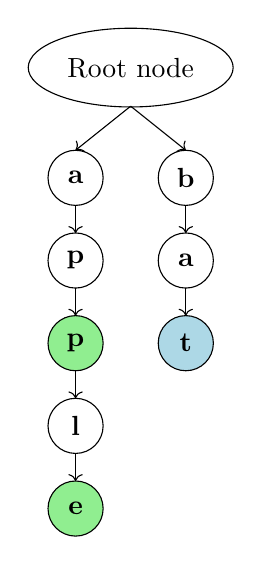
\begin{tikzpicture}[scale=0.7]
    % Vẽ hình elips chứa "Root node" tại tọa độ (0,0)
    \node[ellipse, draw, minimum width=2cm, minimum height=1cm] at (1,0) {Root node};
    
    % Vẽ vòng tròn chứa "a" tại (0,-2), không tô màu
     \fill[green] (0,-5) circle (0.5cm);
    \draw (0,-2) circle (0.5cm);
    \node at (0,-2) {\textbf{a}}; % Chữ "a" in đậm ở tâm vòng tròn
    \draw[->] (1,-0.7) -- (0,-1.5); % Mũi tên từ dưới "Root node" tới trên "a"
    
    % Vẽ vòng tròn chứa "p" thứ nhất tại (0,-3.5), không tô màu
    \draw (0,-3.5) circle (0.5cm);
    \node at (0,-3.5) {\textbf{p}}; % Chữ "p" in đậm ở tâm vòng tròn
    \draw[->] (0,-2.5) -- (0,-3); % Mũi tên từ dưới "a" tới trên "p"
    
    % Vẽ vòng tròn chứa "p" thứ hai tại (0,-5), không tô màu
    \draw (0,-5) circle (0.5cm);
    \node at (0,-5) {\textbf{p}}; % Chữ "p" in đậm ở tâm vòng tròn
    \draw[->] (0,-4) -- (0,-4.5); % Mũi tên từ dưới "p" trước tới trên "p"
    
    % Vẽ vòng tròn chứa "l" tại (0,-6.5), không tô màu
    \draw (0,-6.5) circle (0.5cm);
    \node at (0,-6.5) {\textbf{l}}; % Chữ "l" in đậm ở tâm vòng tròn
    \draw[->] (0,-5.5) -- (0,-6); % Mũi tên từ dưới "p" tới trên "l"
    
    % Vẽ vòng tròn chứa "e" tại (0,-8), tô màu xanh dương
    \fill[green] (0,-8) circle (0.5cm); % Tô nền màu xanh dương
    \draw (0,-8) circle (0.5cm); % Vẽ viền vòng tròn
    \node at (0,-8) {\textbf{e}}; % Chữ "e" in đậm ở tâm vòng tròn
    \draw[->] (0,-7) -- (0,-7.5); % Mũi tên từ dưới "l" tới trên "e"

    %b
     \fill[blue] (2,-5) circle (0.5cm);
    \draw (2,-2) circle (0.5cm);
    \node at (2,-2) {\textbf{b}}; % Chữ "a" in đậm ở tâm vòng tròn
    \draw[->] (1,-0.7) -- (2,-1.5); % Mũi tên từ dưới "Root node" tới trên "a"
    %a
    \draw (2,-3.5) circle (0.5cm);
    \node at (2,-3.5) {\textbf{a}}; % Chữ "a" in đậm ở tâm vòng tròn
    \draw[->] (2,-2.5) -- (2,-3); % Mũi tên từ dưới "Root node" tới trên "a"
    %t
    %\fill[green] (2,-5) circle (0.5cm);
    \draw (2,-5) circle (0.5cm);
    \node at (2,-5) {\textbf{t}}; % Chữ "p" in đậm ở tâm vòng tròn
    \draw[->] (2,-4) -- (2,-4.5); % Mũi tên từ dưới "p" trước tới trên "p"
    
    
\end{tikzpicture}
\end{center}
\end{frame}
\begin{frame}{Insert "batman"}
\begin{center}
    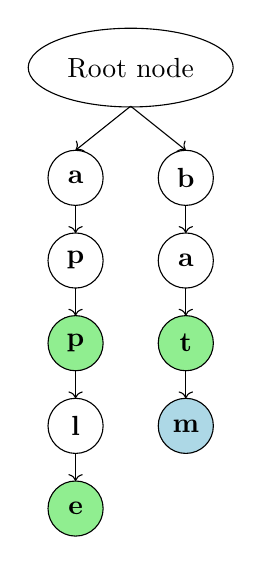
\begin{tikzpicture}[scale=0.7]
    % Vẽ hình elips chứa "Root node" tại tọa độ (0,0)
    \node[ellipse, draw, minimum width=2cm, minimum height=1cm] at (1,0) {Root node};
    
    % Vẽ vòng tròn chứa "a" tại (0,-2), không tô màu
     \fill[green] (0,-5) circle (0.5cm);
    \draw (0,-2) circle (0.5cm);
    \node at (0,-2) {\textbf{a}}; % Chữ "a" in đậm ở tâm vòng tròn
    \draw[->] (1,-0.7) -- (0,-1.5); % Mũi tên từ dưới "Root node" tới trên "a"
    
    % Vẽ vòng tròn chứa "p" thứ nhất tại (0,-3.5), không tô màu
    \draw (0,-3.5) circle (0.5cm);
    \node at (0,-3.5) {\textbf{p}}; % Chữ "p" in đậm ở tâm vòng tròn
    \draw[->] (0,-2.5) -- (0,-3); % Mũi tên từ dưới "a" tới trên "p"
    
    % Vẽ vòng tròn chứa "p" thứ hai tại (0,-5), không tô màu
    \draw (0,-5) circle (0.5cm);
    \node at (0,-5) {\textbf{p}}; % Chữ "p" in đậm ở tâm vòng tròn
    \draw[->] (0,-4) -- (0,-4.5); % Mũi tên từ dưới "p" trước tới trên "p"
    
    % Vẽ vòng tròn chứa "l" tại (0,-6.5), không tô màu
    \draw (0,-6.5) circle (0.5cm);
    \node at (0,-6.5) {\textbf{l}}; % Chữ "l" in đậm ở tâm vòng tròn
    \draw[->] (0,-5.5) -- (0,-6); % Mũi tên từ dưới "p" tới trên "l"
    
    % Vẽ vòng tròn chứa "e" tại (0,-8), tô màu xanh dương
    \fill[green] (0,-8) circle (0.5cm); % Tô nền màu xanh dương
    \draw (0,-8) circle (0.5cm); % Vẽ viền vòng tròn
    \node at (0,-8) {\textbf{e}}; % Chữ "e" in đậm ở tâm vòng tròn
    \draw[->] (0,-7) -- (0,-7.5); % Mũi tên từ dưới "l" tới trên "e"

    %b
    \draw (2,-2) circle (0.5cm);
    \node at (2,-2) {\textbf{b}}; % Chữ "a" in đậm ở tâm vòng tròn
    \draw[->] (1,-0.7) -- (2,-1.5); % Mũi tên từ dưới "Root node" tới trên "a"
    %a
    \draw (2,-3.5) circle (0.5cm);
    \node at (2,-3.5) {\textbf{a}}; % Chữ "a" in đậm ở tâm vòng tròn
    \draw[->] (2,-2.5) -- (2,-3); % Mũi tên từ dưới "Root node" tới trên "a"
    %t
    \fill[green] (2,-5) circle (0.5cm);
    \draw (2,-5) circle (0.5cm);
    \node at (2,-5) {\textbf{t}}; % Chữ "p" in đậm ở tâm vòng tròn
    \draw[->] (2,-4) -- (2,-4.5); % Mũi tên từ dưới "p" trước tới trên "p"
    %m
    \fill[blue] (2,-6.5) circle (0.5cm);
    \draw (2,-6.5) circle (0.5cm);
    \node at (2,-6.5) {\textbf{m}}; % Chữ "l" in đậm ở tâm vòng tròn
    \draw[->] (2,-5.5) -- (2,-6); % Mũi tên từ dưới "p" tới trên "l"

\end{tikzpicture}
\end{center}
\end{frame}
\begin{frame}{Insert "batman"}
\begin{center}
    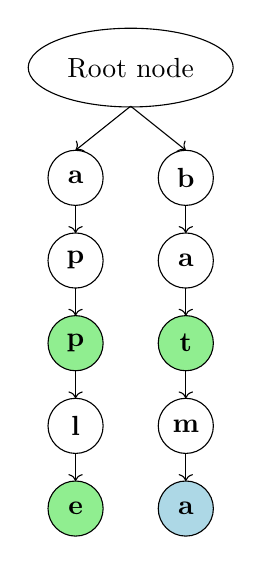
\begin{tikzpicture}[scale=0.7]
    % Vẽ hình elips chứa "Root node" tại tọa độ (0,0)
    \node[ellipse, draw, minimum width=2cm, minimum height=1cm] at (1,0) {Root node};
    
    % Vẽ vòng tròn chứa "a" tại (0,-2), không tô màu
     \fill[green] (0,-5) circle (0.5cm);
    \draw (0,-2) circle (0.5cm);
    \node at (0,-2) {\textbf{a}}; % Chữ "a" in đậm ở tâm vòng tròn
    \draw[->] (1,-0.7) -- (0,-1.5); % Mũi tên từ dưới "Root node" tới trên "a"
    
    % Vẽ vòng tròn chứa "p" thứ nhất tại (0,-3.5), không tô màu
    \draw (0,-3.5) circle (0.5cm);
    \node at (0,-3.5) {\textbf{p}}; % Chữ "p" in đậm ở tâm vòng tròn
    \draw[->] (0,-2.5) -- (0,-3); % Mũi tên từ dưới "a" tới trên "p"
    
    % Vẽ vòng tròn chứa "p" thứ hai tại (0,-5), không tô màu
    \draw (0,-5) circle (0.5cm);
    \node at (0,-5) {\textbf{p}}; % Chữ "p" in đậm ở tâm vòng tròn
    \draw[->] (0,-4) -- (0,-4.5); % Mũi tên từ dưới "p" trước tới trên "p"
    
    % Vẽ vòng tròn chứa "l" tại (0,-6.5), không tô màu
    \draw (0,-6.5) circle (0.5cm);
    \node at (0,-6.5) {\textbf{l}}; % Chữ "l" in đậm ở tâm vòng tròn
    \draw[->] (0,-5.5) -- (0,-6); % Mũi tên từ dưới "p" tới trên "l"
    
    % Vẽ vòng tròn chứa "e" tại (0,-8), tô màu xanh dương
    \fill[green] (0,-8) circle (0.5cm); % Tô nền màu xanh dương
    \draw (0,-8) circle (0.5cm); % Vẽ viền vòng tròn
    \node at (0,-8) {\textbf{e}}; % Chữ "e" in đậm ở tâm vòng tròn
    \draw[->] (0,-7) -- (0,-7.5); % Mũi tên từ dưới "l" tới trên "e"

    %b
    \draw (2,-2) circle (0.5cm);
    \node at (2,-2) {\textbf{b}}; % Chữ "a" in đậm ở tâm vòng tròn
    \draw[->] (1,-0.7) -- (2,-1.5); % Mũi tên từ dưới "Root node" tới trên "a"
    %a
    \draw (2,-3.5) circle (0.5cm);
    \node at (2,-3.5) {\textbf{a}}; % Chữ "a" in đậm ở tâm vòng tròn
    \draw[->] (2,-2.5) -- (2,-3); % Mũi tên từ dưới "Root node" tới trên "a"
    %t
    \fill[green] (2,-5) circle (0.5cm);
    \draw (2,-5) circle (0.5cm);
    \node at (2,-5) {\textbf{t}}; % Chữ "p" in đậm ở tâm vòng tròn
    \draw[->] (2,-4) -- (2,-4.5); % Mũi tên từ dưới "p" trước tới trên "p"
    %m
    \draw (2,-6.5) circle (0.5cm);
    \node at (2,-6.5) {\textbf{m}}; % Chữ "l" in đậm ở tâm vòng tròn
    \draw[->] (2,-5.5) -- (2,-6); % Mũi tên từ dưới "p" tới trên "l"
    %a
     \fill[blue] (2,-8) circle (0.5cm); % Tô nền màu xanh dương
    \draw (02,-8) circle (0.5cm); % Vẽ viền vòng tròn
    \node at (02,-8) {\textbf{a}}; % Chữ "e" in đậm ở tâm vòng tròn
    \draw[->] (02,-7) -- (02,-7.5); % Mũi tên từ dưới "l" tới trên "e"
    
    
\end{tikzpicture}
\end{center}
\end{frame}
\begin{frame}{Insert "batman"}
\begin{center}
    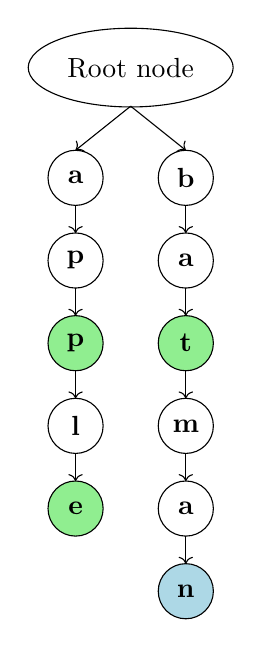
\begin{tikzpicture}[scale=0.7]
    % Vẽ hình elips chứa "Root node" tại tọa độ (0,0)
    \node[ellipse, draw, minimum width=2cm, minimum height=1cm] at (1,0) {Root node};
    
    % Vẽ vòng tròn chứa "a" tại (0,-2), không tô màu
     \fill[green] (0,-5) circle (0.5cm);
    \draw (0,-2) circle (0.5cm);
    \node at (0,-2) {\textbf{a}}; % Chữ "a" in đậm ở tâm vòng tròn
    \draw[->] (1,-0.7) -- (0,-1.5); % Mũi tên từ dưới "Root node" tới trên "a"
    
    % Vẽ vòng tròn chứa "p" thứ nhất tại (0,-3.5), không tô màu
    \draw (0,-3.5) circle (0.5cm);
    \node at (0,-3.5) {\textbf{p}}; % Chữ "p" in đậm ở tâm vòng tròn
    \draw[->] (0,-2.5) -- (0,-3); % Mũi tên từ dưới "a" tới trên "p"
    
    % Vẽ vòng tròn chứa "p" thứ hai tại (0,-5), không tô màu
    \draw (0,-5) circle (0.5cm);
    \node at (0,-5) {\textbf{p}}; % Chữ "p" in đậm ở tâm vòng tròn
    \draw[->] (0,-4) -- (0,-4.5); % Mũi tên từ dưới "p" trước tới trên "p"
    
    % Vẽ vòng tròn chứa "l" tại (0,-6.5), không tô màu
    \draw (0,-6.5) circle (0.5cm);
    \node at (0,-6.5) {\textbf{l}}; % Chữ "l" in đậm ở tâm vòng tròn
    \draw[->] (0,-5.5) -- (0,-6); % Mũi tên từ dưới "p" tới trên "l"
    
    % Vẽ vòng tròn chứa "e" tại (0,-8), tô màu xanh dương
    \fill[green] (0,-8) circle (0.5cm); % Tô nền màu xanh dương
    \draw (0,-8) circle (0.5cm); % Vẽ viền vòng tròn
    \node at (0,-8) {\textbf{e}}; % Chữ "e" in đậm ở tâm vòng tròn
    \draw[->] (0,-7) -- (0,-7.5); % Mũi tên từ dưới "l" tới trên "e"

    %b
    \draw (2,-2) circle (0.5cm);
    \node at (2,-2) {\textbf{b}}; % Chữ "a" in đậm ở tâm vòng tròn
    \draw[->] (1,-0.7) -- (2,-1.5); % Mũi tên từ dưới "Root node" tới trên "a"
    %a
    \draw (2,-3.5) circle (0.5cm);
    \node at (2,-3.5) {\textbf{a}}; % Chữ "a" in đậm ở tâm vòng tròn
    \draw[->] (2,-2.5) -- (2,-3); % Mũi tên từ dưới "Root node" tới trên "a"
    %t
    \fill[green] (2,-5) circle (0.5cm);
    \draw (2,-5) circle (0.5cm);
    \node at (2,-5) {\textbf{t}}; % Chữ "p" in đậm ở tâm vòng tròn
    \draw[->] (2,-4) -- (2,-4.5); % Mũi tên từ dưới "p" trước tới trên "p"
    %m
    \draw (2,-6.5) circle (0.5cm);
    \node at (2,-6.5) {\textbf{m}}; % Chữ "l" in đậm ở tâm vòng tròn
    \draw[->] (2,-5.5) -- (2,-6); % Mũi tên từ dưới "p" tới trên "l"
    %a
    \draw (02,-8) circle (0.5cm); % Vẽ viền vòng tròn
    \node at (02,-8) {\textbf{a}}; % Chữ "e" in đậm ở tâm vòng tròn
    \draw[->] (02,-7) -- (02,-7.5); % Mũi tên từ dưới "l" tới trên "e"
    %n
    \fill[blue] (2,-9.5) circle (0.5cm); % Tô nền màu xanh dương
    \draw (02,-9.5) circle (0.5cm); % Vẽ viền vòng tròn
    \node at (02,-9.5) {\textbf{n}}; % Chữ "e" in đậm ở tâm vòng tròn
    \draw[->] (02,-8.5) -- (02,-9); % Mũi tên từ dưới "l" tới trên "e"
    
    
\end{tikzpicture}
\end{center}
\end{frame}

\begin{frame}{Insert "batman"}
\begin{center}
    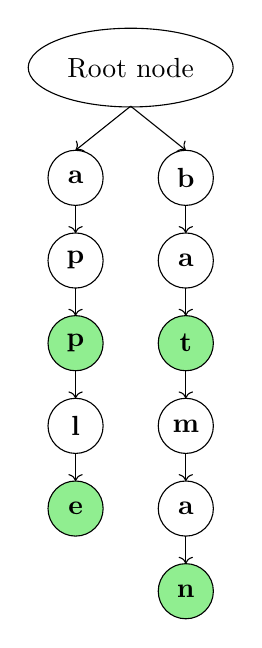
\begin{tikzpicture}[scale=0.7]
    % Vẽ hình elips chứa "Root node" tại tọa độ (0,0)
    \node[ellipse, draw, minimum width=2cm, minimum height=1cm] at (1,0) {Root node};
    
    % Vẽ vòng tròn chứa "a" tại (0,-2), không tô màu
     \fill[green] (0,-5) circle (0.5cm);
    \draw (0,-2) circle (0.5cm);
    \node at (0,-2) {\textbf{a}}; % Chữ "a" in đậm ở tâm vòng tròn
    \draw[->] (1,-0.7) -- (0,-1.5); % Mũi tên từ dưới "Root node" tới trên "a"
    
    % Vẽ vòng tròn chứa "p" thứ nhất tại (0,-3.5), không tô màu
    \draw (0,-3.5) circle (0.5cm);
    \node at (0,-3.5) {\textbf{p}}; % Chữ "p" in đậm ở tâm vòng tròn
    \draw[->] (0,-2.5) -- (0,-3); % Mũi tên từ dưới "a" tới trên "p"
    
    % Vẽ vòng tròn chứa "p" thứ hai tại (0,-5), không tô màu
    \draw (0,-5) circle (0.5cm);
    \node at (0,-5) {\textbf{p}}; % Chữ "p" in đậm ở tâm vòng tròn
    \draw[->] (0,-4) -- (0,-4.5); % Mũi tên từ dưới "p" trước tới trên "p"
    
    % Vẽ vòng tròn chứa "l" tại (0,-6.5), không tô màu
    \draw (0,-6.5) circle (0.5cm);
    \node at (0,-6.5) {\textbf{l}}; % Chữ "l" in đậm ở tâm vòng tròn
    \draw[->] (0,-5.5) -- (0,-6); % Mũi tên từ dưới "p" tới trên "l"
    
    % Vẽ vòng tròn chứa "e" tại (0,-8), tô màu xanh dương
    \fill[green] (0,-8) circle (0.5cm); % Tô nền màu xanh dương
    \draw (0,-8) circle (0.5cm); % Vẽ viền vòng tròn
    \node at (0,-8) {\textbf{e}}; % Chữ "e" in đậm ở tâm vòng tròn
    \draw[->] (0,-7) -- (0,-7.5); % Mũi tên từ dưới "l" tới trên "e"

    %b
    \draw (2,-2) circle (0.5cm);
    \node at (2,-2) {\textbf{b}}; % Chữ "a" in đậm ở tâm vòng tròn
    \draw[->] (1,-0.7) -- (2,-1.5); % Mũi tên từ dưới "Root node" tới trên "a"
    %a
    \draw (2,-3.5) circle (0.5cm);
    \node at (2,-3.5) {\textbf{a}}; % Chữ "a" in đậm ở tâm vòng tròn
    \draw[->] (2,-2.5) -- (2,-3); % Mũi tên từ dưới "Root node" tới trên "a"
    %t
    \fill[green] (2,-5) circle (0.5cm);
    \draw (2,-5) circle (0.5cm);
    \node at (2,-5) {\textbf{t}}; % Chữ "p" in đậm ở tâm vòng tròn
    \draw[->] (2,-4) -- (2,-4.5); % Mũi tên từ dưới "p" trước tới trên "p"
    %m
    \draw (2,-6.5) circle (0.5cm);
    \node at (2,-6.5) {\textbf{m}}; % Chữ "l" in đậm ở tâm vòng tròn
    \draw[->] (2,-5.5) -- (2,-6); % Mũi tên từ dưới "p" tới trên "l"
    %a
    \draw (02,-8) circle (0.5cm); % Vẽ viền vòng tròn
    \node at (02,-8) {\textbf{a}}; % Chữ "e" in đậm ở tâm vòng tròn
    \draw[->] (02,-7) -- (02,-7.5); % Mũi tên từ dưới "l" tới trên "e"
    %n
    \fill[green] (2,-9.5) circle (0.5cm); % Tô nền màu xanh dương
    \draw (02,-9.5) circle (0.5cm); % Vẽ viền vòng tròn
    \node at (02,-9.5) {\textbf{n}}; % Chữ "e" in đậm ở tâm vòng tròn
    \draw[->] (02,-8.5) -- (02,-9); % Mũi tên từ dưới "l" tới trên "e"
\end{tikzpicture}
\end{center}
\end{frame}
\begin{frame}{Insert "base"}
\begin{center}
    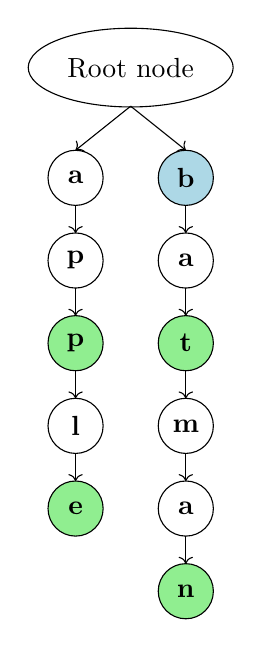
\begin{tikzpicture}[scale=0.7]
    % Vẽ hình elips chứa "Root node" tại tọa độ (0,0)
    \node[ellipse, draw, minimum width=2cm, minimum height=1cm] at (1,0) {Root node};
    
    % Vẽ vòng tròn chứa "a" tại (0,-2), không tô màu
     \fill[green] (0,-5) circle (0.5cm);
    \draw (0,-2) circle (0.5cm);
    \node at (0,-2) {\textbf{a}}; % Chữ "a" in đậm ở tâm vòng tròn
    \draw[->] (1,-0.7) -- (0,-1.5); % Mũi tên từ dưới "Root node" tới trên "a"
    
    % Vẽ vòng tròn chứa "p" thứ nhất tại (0,-3.5), không tô màu
    \draw (0,-3.5) circle (0.5cm);
    \node at (0,-3.5) {\textbf{p}}; % Chữ "p" in đậm ở tâm vòng tròn
    \draw[->] (0,-2.5) -- (0,-3); % Mũi tên từ dưới "a" tới trên "p"
    
    % Vẽ vòng tròn chứa "p" thứ hai tại (0,-5), không tô màu
    \draw (0,-5) circle (0.5cm);
    \node at (0,-5) {\textbf{p}}; % Chữ "p" in đậm ở tâm vòng tròn
    \draw[->] (0,-4) -- (0,-4.5); % Mũi tên từ dưới "p" trước tới trên "p"
    
    % Vẽ vòng tròn chứa "l" tại (0,-6.5), không tô màu
    \draw (0,-6.5) circle (0.5cm);
    \node at (0,-6.5) {\textbf{l}}; % Chữ "l" in đậm ở tâm vòng tròn
    \draw[->] (0,-5.5) -- (0,-6); % Mũi tên từ dưới "p" tới trên "l"
    
    % Vẽ vòng tròn chứa "e" tại (0,-8), tô màu xanh dương
    \fill[green] (0,-8) circle (0.5cm); % Tô nền màu xanh dương
    \draw (0,-8) circle (0.5cm); % Vẽ viền vòng tròn
    \node at (0,-8) {\textbf{e}}; % Chữ "e" in đậm ở tâm vòng tròn
    \draw[->] (0,-7) -- (0,-7.5); % Mũi tên từ dưới "l" tới trên "e"

    %b
       \fill[blue] (2,-2) circle (0.5cm);
    \draw (2,-2) circle (0.5cm);
    \node at (2,-2) {\textbf{b}}; % Chữ "a" in đậm ở tâm vòng tròn
    \draw[->] (1,-0.7) -- (2,-1.5); % Mũi tên từ dưới "Root node" tới trên "a"
    %a
    \draw (2,-3.5) circle (0.5cm);
    \node at (2,-3.5) {\textbf{a}}; % Chữ "a" in đậm ở tâm vòng tròn
    \draw[->] (2,-2.5) -- (2,-3); % Mũi tên từ dưới "Root node" tới trên "a"
    %t
    \fill[green] (2,-5) circle (0.5cm);
    \draw (2,-5) circle (0.5cm);
    \node at (2,-5) {\textbf{t}}; % Chữ "p" in đậm ở tâm vòng tròn
    \draw[->] (2,-4) -- (2,-4.5); % Mũi tên từ dưới "p" trước tới trên "p"
    %m
    \draw (2,-6.5) circle (0.5cm);
    \node at (2,-6.5) {\textbf{m}}; % Chữ "l" in đậm ở tâm vòng tròn
    \draw[->] (2,-5.5) -- (2,-6); % Mũi tên từ dưới "p" tới trên "l"
    %a
    \draw (02,-8) circle (0.5cm); % Vẽ viền vòng tròn
    \node at (02,-8) {\textbf{a}}; % Chữ "e" in đậm ở tâm vòng tròn
    \draw[->] (02,-7) -- (02,-7.5); % Mũi tên từ dưới "l" tới trên "e"
    %n
    \fill[green] (2,-9.5) circle (0.5cm); % Tô nền màu xanh dương
    \draw (02,-9.5) circle (0.5cm); % Vẽ viền vòng tròn
    \node at (02,-9.5) {\textbf{n}}; % Chữ "e" in đậm ở tâm vòng tròn
    \draw[->] (02,-8.5) -- (02,-9); % Mũi tên từ dưới "l" tới trên "e"
\end{tikzpicture}
\end{center}
\end{frame}
\begin{frame}{Insert "base"}
\begin{center}
    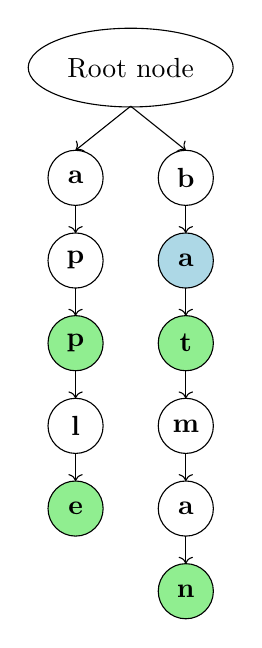
\begin{tikzpicture}[scale=0.7]
    % Vẽ hình elips chứa "Root node" tại tọa độ (0,0)
    \node[ellipse, draw, minimum width=2cm, minimum height=1cm] at (1,0) {Root node};
    
    % Vẽ vòng tròn chứa "a" tại (0,-2), không tô màu
     \fill[green] (0,-5) circle (0.5cm);
    \draw (0,-2) circle (0.5cm);
    \node at (0,-2) {\textbf{a}}; % Chữ "a" in đậm ở tâm vòng tròn
    \draw[->] (1,-0.7) -- (0,-1.5); % Mũi tên từ dưới "Root node" tới trên "a"
    
    % Vẽ vòng tròn chứa "p" thứ nhất tại (0,-3.5), không tô màu
    \draw (0,-3.5) circle (0.5cm);
    \node at (0,-3.5) {\textbf{p}}; % Chữ "p" in đậm ở tâm vòng tròn
    \draw[->] (0,-2.5) -- (0,-3); % Mũi tên từ dưới "a" tới trên "p"
    
    % Vẽ vòng tròn chứa "p" thứ hai tại (0,-5), không tô màu
    \draw (0,-5) circle (0.5cm);
    \node at (0,-5) {\textbf{p}}; % Chữ "p" in đậm ở tâm vòng tròn
    \draw[->] (0,-4) -- (0,-4.5); % Mũi tên từ dưới "p" trước tới trên "p"
    
    % Vẽ vòng tròn chứa "l" tại (0,-6.5), không tô màu
    \draw (0,-6.5) circle (0.5cm);
    \node at (0,-6.5) {\textbf{l}}; % Chữ "l" in đậm ở tâm vòng tròn
    \draw[->] (0,-5.5) -- (0,-6); % Mũi tên từ dưới "p" tới trên "l"
    
    % Vẽ vòng tròn chứa "e" tại (0,-8), tô màu xanh dương
    \fill[green] (0,-8) circle (0.5cm); % Tô nền màu xanh dương
    \draw (0,-8) circle (0.5cm); % Vẽ viền vòng tròn
    \node at (0,-8) {\textbf{e}}; % Chữ "e" in đậm ở tâm vòng tròn
    \draw[->] (0,-7) -- (0,-7.5); % Mũi tên từ dưới "l" tới trên "e"

    %b
       \fill[blue] (2,-3.5) circle (0.5cm);
    \draw (2,-2) circle (0.5cm);
    \node at (2,-2) {\textbf{b}}; % Chữ "a" in đậm ở tâm vòng tròn
    \draw[->] (1,-0.7) -- (2,-1.5); % Mũi tên từ dưới "Root node" tới trên "a"
    %a
    \draw (2,-3.5) circle (0.5cm);
    \node at (2,-3.5) {\textbf{a}}; % Chữ "a" in đậm ở tâm vòng tròn
    \draw[->] (2,-2.5) -- (2,-3); % Mũi tên từ dưới "Root node" tới trên "a"
    %t
    \fill[green] (2,-5) circle (0.5cm);
    \draw (2,-5) circle (0.5cm);
    \node at (2,-5) {\textbf{t}}; % Chữ "p" in đậm ở tâm vòng tròn
    \draw[->] (2,-4) -- (2,-4.5); % Mũi tên từ dưới "p" trước tới trên "p"
    %m
    \draw (2,-6.5) circle (0.5cm);
    \node at (2,-6.5) {\textbf{m}}; % Chữ "l" in đậm ở tâm vòng tròn
    \draw[->] (2,-5.5) -- (2,-6); % Mũi tên từ dưới "p" tới trên "l"
    %a
    \draw (02,-8) circle (0.5cm); % Vẽ viền vòng tròn
    \node at (02,-8) {\textbf{a}}; % Chữ "e" in đậm ở tâm vòng tròn
    \draw[->] (02,-7) -- (02,-7.5); % Mũi tên từ dưới "l" tới trên "e"
    %n
    \fill[green] (2,-9.5) circle (0.5cm); % Tô nền màu xanh dương
    \draw (02,-9.5) circle (0.5cm); % Vẽ viền vòng tròn
    \node at (02,-9.5) {\textbf{n}}; % Chữ "e" in đậm ở tâm vòng tròn
    \draw[->] (02,-8.5) -- (02,-9); % Mũi tên từ dưới "l" tới trên "e"
\end{tikzpicture}
\end{center}
\end{frame}
\begin{frame}{Insert "base"}
\begin{center}
    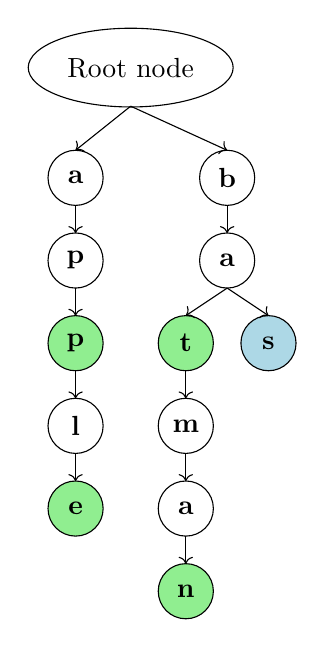
\begin{tikzpicture}[scale=0.7]
    % Vẽ hình elips chứa "Root node" tại tọa độ (0,0)
    \node[ellipse, draw, minimum width=2cm, minimum height=1cm] at (1,0) {Root node};
    
    % Vẽ vòng tròn chứa "a" tại (0,-2), không tô màu
     \fill[green] (0,-5) circle (0.5cm);
    \draw (0,-2) circle (0.5cm);
    \node at (0,-2) {\textbf{a}}; % Chữ "a" in đậm ở tâm vòng tròn
    \draw[->] (1,-0.7) -- (0,-1.5); % Mũi tên từ dưới "Root node" tới trên "a"
    
    % Vẽ vòng tròn chứa "p" thứ nhất tại (0,-3.5), không tô màu
    \draw (0,-3.5) circle (0.5cm);
    \node at (0,-3.5) {\textbf{p}}; % Chữ "p" in đậm ở tâm vòng tròn
    \draw[->] (0,-2.5) -- (0,-3); % Mũi tên từ dưới "a" tới trên "p"
    
    % Vẽ vòng tròn chứa "p" thứ hai tại (0,-5), không tô màu
    \draw (0,-5) circle (0.5cm);
    \node at (0,-5) {\textbf{p}}; % Chữ "p" in đậm ở tâm vòng tròn
    \draw[->] (0,-4) -- (0,-4.5); % Mũi tên từ dưới "p" trước tới trên "p"
    
    % Vẽ vòng tròn chứa "l" tại (0,-6.5), không tô màu
    \draw (0,-6.5) circle (0.5cm);
    \node at (0,-6.5) {\textbf{l}}; % Chữ "l" in đậm ở tâm vòng tròn
    \draw[->] (0,-5.5) -- (0,-6); % Mũi tên từ dưới "p" tới trên "l"
    
    % Vẽ vòng tròn chứa "e" tại (0,-8), tô màu xanh dương
    \fill[green] (0,-8) circle (0.5cm); % Tô nền màu xanh dương
    \draw (0,-8) circle (0.5cm); % Vẽ viền vòng tròn
    \node at (0,-8) {\textbf{e}}; % Chữ "e" in đậm ở tâm vòng tròn
    \draw[->] (0,-7) -- (0,-7.5); % Mũi tên từ dưới "l" tới trên "e"

    %b
    \draw (2.75,-2) circle (0.5cm);
    \node at (2.75,-2) {\textbf{b}}; % Chữ "a" in đậm ở tâm vòng tròn
    \draw[->] (1,-0.7) -- (2.75,-1.5); % Mũi tên từ dưới "Root node" tới trên "a"
    %a
    \draw (2.75,-3.5) circle (0.5cm);
    \node at (2.75,-3.5) {\textbf{a}}; % Chữ "a" in đậm ở tâm vòng tròn
    \draw[->] (2.75,-2.5) -- (2.75,-3); % Mũi tên từ dưới "Root node" tới trên
    %s
    \fill[blue] (3.5,-5) circle (0.5cm);
    \draw (3.5,-5) circle (0.5cm);
    \node at (3.5,-5) {\textbf{s}}; % Chữ "p" in đậm ở tâm vòng tròn
    \draw[->] (2.75,-4) -- (3.5,-4.5); % Mũi tên từ dưới "p" trước tới trên "p"
    %t
    \fill[green] (2,-5) circle (0.5cm);
    \draw (2,-5) circle (0.5cm);
    \node at (2,-5) {\textbf{t}}; % Chữ "p" in đậm ở tâm vòng tròn
    \draw[->] (2.75,-4) -- (2,-4.5); % Mũi tên từ dưới "p" trước tới trên "p"
    %m
    \draw (2,-6.5) circle (0.5cm);
    \node at (2,-6.5) {\textbf{m}}; % Chữ "l" in đậm ở tâm vòng tròn
    \draw[->] (2,-5.5) -- (2,-6); % Mũi tên từ dưới "p" tới trên "l"
    %a
    \draw (02,-8) circle (0.5cm); % Vẽ viền vòng tròn
    \node at (02,-8) {\textbf{a}}; % Chữ "e" in đậm ở tâm vòng tròn
    \draw[->] (02,-7) -- (02,-7.5); % Mũi tên từ dưới "l" tới trên "e"
    %n
    \fill[green] (2,-9.5) circle (0.5cm); % Tô nền màu xanh dương
    \draw (02,-9.5) circle (0.5cm); % Vẽ viền vòng tròn
    \node at (02,-9.5) {\textbf{n}}; % Chữ "e" in đậm ở tâm vòng tròn
    \draw[->] (02,-8.5) -- (02,-9); % Mũi tên từ dưới "l" tới trên "e"
\end{tikzpicture}
\end{center}
\end{frame}
\begin{frame}{Insert "base"}
\begin{center}
    
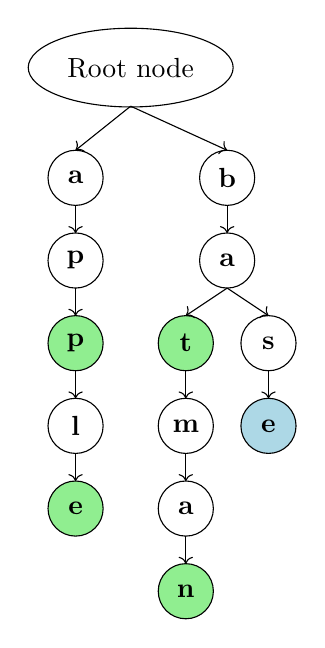
\begin{tikzpicture}[scale=0.7]
    % Vẽ hình elips chứa "Root node" tại tọa độ (0,0)
    \node[ellipse, draw, minimum width=2cm, minimum height=1cm] at (1,0) {Root node};
    
    % Vẽ vòng tròn chứa "a" tại (0,-2), không tô màu
     \fill[green] (0,-5) circle (0.5cm);
    \draw (0,-2) circle (0.5cm);
    \node at (0,-2) {\textbf{a}}; % Chữ "a" in đậm ở tâm vòng tròn
    \draw[->] (1,-0.7) -- (0,-1.5); % Mũi tên từ dưới "Root node" tới trên "a"
    
    % Vẽ vòng tròn chứa "p" thứ nhất tại (0,-3.5), không tô màu
    \draw (0,-3.5) circle (0.5cm);
    \node at (0,-3.5) {\textbf{p}}; % Chữ "p" in đậm ở tâm vòng tròn
    \draw[->] (0,-2.5) -- (0,-3); % Mũi tên từ dưới "a" tới trên "p"
    
    % Vẽ vòng tròn chứa "p" thứ hai tại (0,-5), không tô màu
    \draw (0,-5) circle (0.5cm);
    \node at (0,-5) {\textbf{p}}; % Chữ "p" in đậm ở tâm vòng tròn
    \draw[->] (0,-4) -- (0,-4.5); % Mũi tên từ dưới "p" trước tới trên "p"
    
    % Vẽ vòng tròn chứa "l" tại (0,-6.5), không tô màu
    \draw (0,-6.5) circle (0.5cm);
    \node at (0,-6.5) {\textbf{l}}; % Chữ "l" in đậm ở tâm vòng tròn
    \draw[->] (0,-5.5) -- (0,-6); % Mũi tên từ dưới "p" tới trên "l"
    
    % Vẽ vòng tròn chứa "e" tại (0,-8), tô màu xanh dương
    \fill[green] (0,-8) circle (0.5cm); % Tô nền màu xanh dương
    \draw (0,-8) circle (0.5cm); % Vẽ viền vòng tròn
    \node at (0,-8) {\textbf{e}}; % Chữ "e" in đậm ở tâm vòng tròn
    \draw[->] (0,-7) -- (0,-7.5); % Mũi tên từ dưới "l" tới trên "e"

    %b
    \draw (2.75,-2) circle (0.5cm);
    \node at (2.75,-2) {\textbf{b}}; % Chữ "a" in đậm ở tâm vòng tròn
    \draw[->] (1,-0.7) -- (2.75,-1.5); % Mũi tên từ dưới "Root node" tới trên "a"
    %a
    \draw (2.75,-3.5) circle (0.5cm);
    \node at (2.75,-3.5) {\textbf{a}}; % Chữ "a" in đậm ở tâm vòng tròn
    \draw[->] (2.75,-2.5) -- (2.75,-3); % Mũi tên từ dưới "Root node" tới trên
    %s
    \draw (3.5,-5) circle (0.5cm);
    \node at (3.5,-5) {\textbf{s}}; % Chữ "p" in đậm ở tâm vòng tròn
    \draw[->] (2.75,-4) -- (3.5,-4.5); % Mũi tên từ dưới "p" trước tới trên "p"
    %e
    \fill[blue] (3.5,-6.5) circle (0.5cm);
     \draw (3.5,-6.5) circle (0.5cm);
    \node at (3.5,-6.5) {\textbf{e}}; % Chữ "l" in đậm ở tâm vòng tròn
    \draw[->] (3.5,-5.5) -- (3.5,-6); % Mũi tên từ dưới "p" tới trên "l"
    %t
    \fill[green] (2,-5) circle (0.5cm);
    \draw (2,-5) circle (0.5cm);
    \node at (2,-5) {\textbf{t}}; % Chữ "p" in đậm ở tâm vòng tròn
    \draw[->] (2.75,-4) -- (2,-4.5); % Mũi tên từ dưới "p" trước tới trên "p"
    %m
    \draw (2,-6.5) circle (0.5cm);
    \node at (2,-6.5) {\textbf{m}}; % Chữ "l" in đậm ở tâm vòng tròn
    \draw[->] (2,-5.5) -- (2,-6); % Mũi tên từ dưới "p" tới trên "l"
    %a
    \draw (02,-8) circle (0.5cm); % Vẽ viền vòng tròn
    \node at (02,-8) {\textbf{a}}; % Chữ "e" in đậm ở tâm vòng tròn
    \draw[->] (02,-7) -- (02,-7.5); % Mũi tên từ dưới "l" tới trên "e"
    %n
    \fill[green] (2,-9.5) circle (0.5cm); % Tô nền màu xanh dương
    \draw (02,-9.5) circle (0.5cm); % Vẽ viền vòng tròn
    \node at (02,-9.5) {\textbf{n}}; % Chữ "e" in đậm ở tâm vòng tròn
    \draw[->] (02,-8.5) -- (02,-9); % Mũi tên từ dưới "l" tới trên "e"
\end{tikzpicture}
\end{center}
\end{frame}
\begin{frame}{Insert "base"}
\begin{center}
    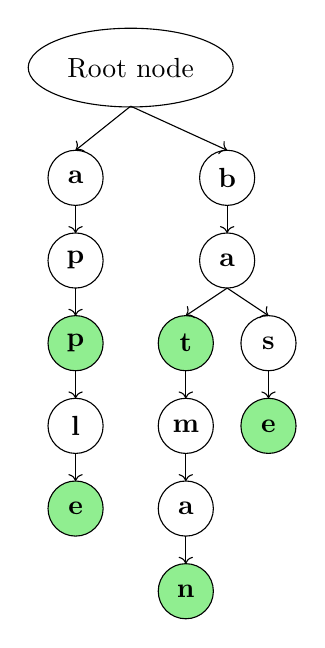
\begin{tikzpicture}[scale=0.7]
    % Vẽ hình elips chứa "Root node" tại tọa độ (0,0)
    \node[ellipse, draw, minimum width=2cm, minimum height=1cm] at (1,0) {Root node};
    
    % Vẽ vòng tròn chứa "a" tại (0,-2), không tô màu
     \fill[green] (0,-5) circle (0.5cm);
    \draw (0,-2) circle (0.5cm);
    \node at (0,-2) {\textbf{a}}; % Chữ "a" in đậm ở tâm vòng tròn
    \draw[->] (1,-0.7) -- (0,-1.5); % Mũi tên từ dưới "Root node" tới trên "a"
    
    % Vẽ vòng tròn chứa "p" thứ nhất tại (0,-3.5), không tô màu
    \draw (0,-3.5) circle (0.5cm);
    \node at (0,-3.5) {\textbf{p}}; % Chữ "p" in đậm ở tâm vòng tròn
    \draw[->] (0,-2.5) -- (0,-3); % Mũi tên từ dưới "a" tới trên "p"
    
    % Vẽ vòng tròn chứa "p" thứ hai tại (0,-5), không tô màu
    \draw (0,-5) circle (0.5cm);
    \node at (0,-5) {\textbf{p}}; % Chữ "p" in đậm ở tâm vòng tròn
    \draw[->] (0,-4) -- (0,-4.5); % Mũi tên từ dưới "p" trước tới trên "p"
    
    % Vẽ vòng tròn chứa "l" tại (0,-6.5), không tô màu
    \draw (0,-6.5) circle (0.5cm);
    \node at (0,-6.5) {\textbf{l}}; % Chữ "l" in đậm ở tâm vòng tròn
    \draw[->] (0,-5.5) -- (0,-6); % Mũi tên từ dưới "p" tới trên "l"
    
    % Vẽ vòng tròn chứa "e" tại (0,-8), tô màu xanh dương
    \fill[green] (0,-8) circle (0.5cm); % Tô nền màu xanh dương
    \draw (0,-8) circle (0.5cm); % Vẽ viền vòng tròn
    \node at (0,-8) {\textbf{e}}; % Chữ "e" in đậm ở tâm vòng tròn
    \draw[->] (0,-7) -- (0,-7.5); % Mũi tên từ dưới "l" tới trên "e"

    %b
    \draw (2.75,-2) circle (0.5cm);
    \node at (2.75,-2) {\textbf{b}}; % Chữ "a" in đậm ở tâm vòng tròn
    \draw[->] (1,-0.7) -- (2.75,-1.5); % Mũi tên từ dưới "Root node" tới trên "a"
    %a
    \draw (2.75,-3.5) circle (0.5cm);
    \node at (2.75,-3.5) {\textbf{a}}; % Chữ "a" in đậm ở tâm vòng tròn
    \draw[->] (2.75,-2.5) -- (2.75,-3); % Mũi tên từ dưới "Root node" tới trên
    %s
    \draw (3.5,-5) circle (0.5cm);
    \node at (3.5,-5) {\textbf{s}}; % Chữ "p" in đậm ở tâm vòng tròn
    \draw[->] (2.75,-4) -- (3.5,-4.5); % Mũi tên từ dưới "p" trước tới trên "p"
    %e
    \fill[green] (3.5,-6.5) circle (0.5cm);
     \draw (3.5,-6.5) circle (0.5cm);
    \node at (3.5,-6.5) {\textbf{e}}; % Chữ "l" in đậm ở tâm vòng tròn
    \draw[->] (3.5,-5.5) -- (3.5,-6); % Mũi tên từ dưới "p" tới trên "l"
    %t
    \fill[green] (2,-5) circle (0.5cm);
    \draw (2,-5) circle (0.5cm);
    \node at (2,-5) {\textbf{t}}; % Chữ "p" in đậm ở tâm vòng tròn
    \draw[->] (2.75,-4) -- (2,-4.5); % Mũi tên từ dưới "p" trước tới trên "p"
    %m
    \draw (2,-6.5) circle (0.5cm);
    \node at (2,-6.5) {\textbf{m}}; % Chữ "l" in đậm ở tâm vòng tròn
    \draw[->] (2,-5.5) -- (2,-6); % Mũi tên từ dưới "p" tới trên "l"
    %a
    \draw (02,-8) circle (0.5cm); % Vẽ viền vòng tròn
    \node at (02,-8) {\textbf{a}}; % Chữ "e" in đậm ở tâm vòng tròn
    \draw[->] (02,-7) -- (02,-7.5); % Mũi tên từ dưới "l" tới trên "e"
    %n
    \fill[green] (2,-9.5) circle (0.5cm); % Tô nền màu xanh dương
    \draw (02,-9.5) circle (0.5cm); % Vẽ viền vòng tròn
    \node at (02,-9.5) {\textbf{n}}; % Chữ "e" in đậm ở tâm vòng tròn
    \draw[->] (02,-8.5) -- (02,-9); % Mũi tên từ dưới "l" tới trên "e"
\end{tikzpicture}
\end{center}
\end{frame}

\begin{frame}{Search: O(L)}
            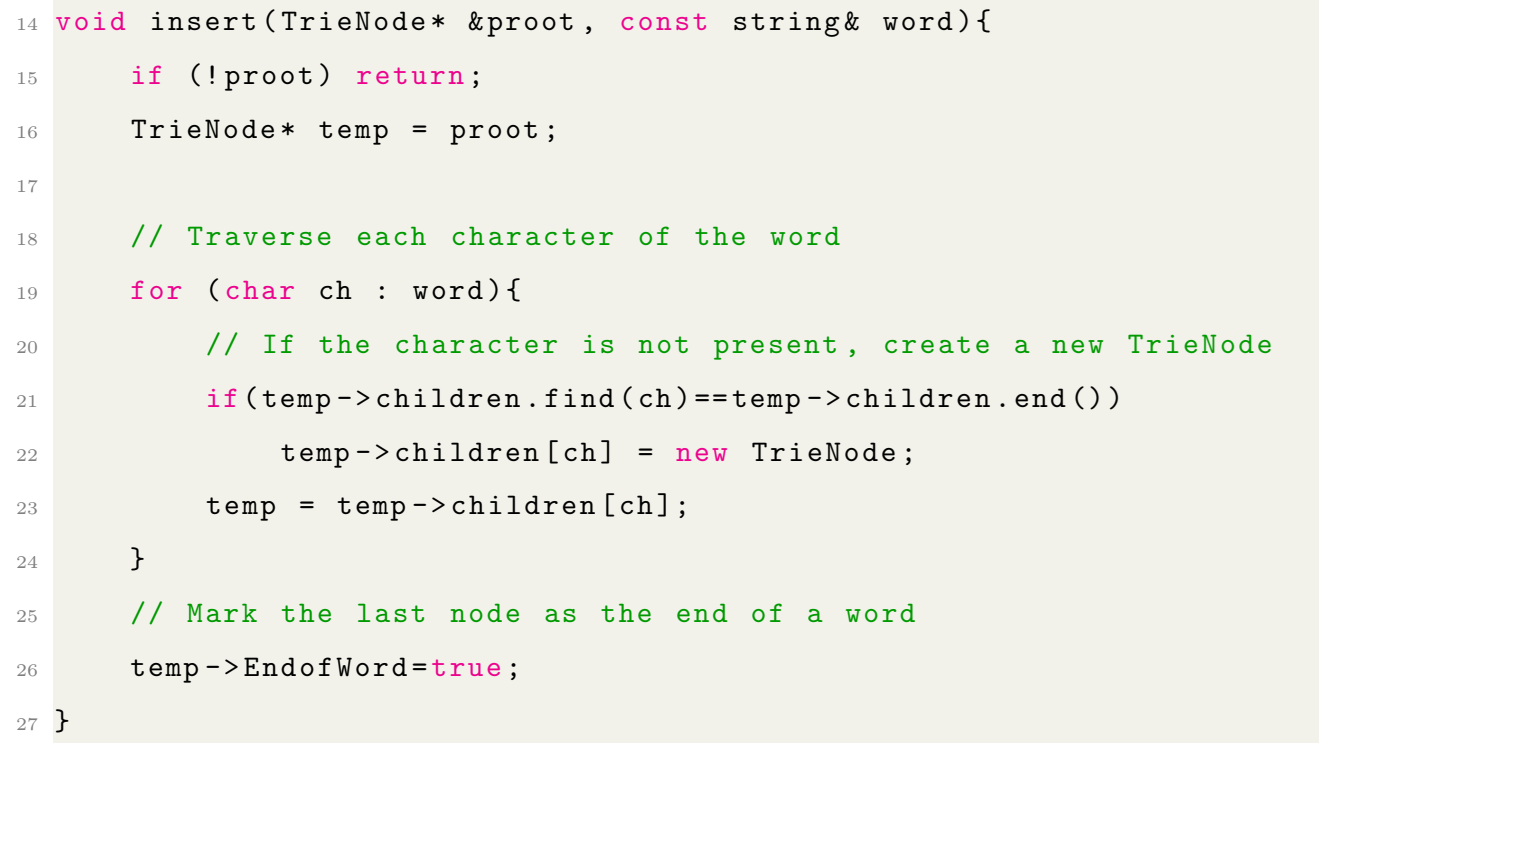
\includegraphics[scale=0.5]{se2.png}
\end{frame}
\begin{frame}{Search "bat"}
    \begin{center}
            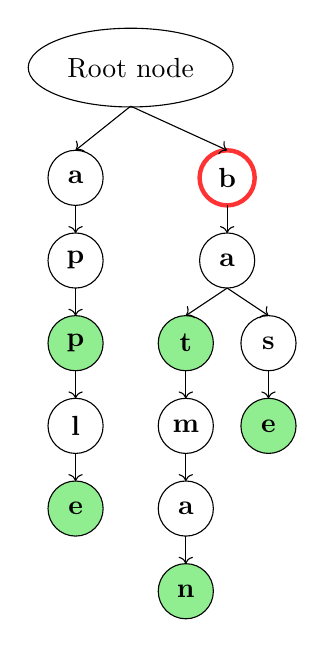
\begin{tikzpicture}[scale=0.7]
    % Vẽ hình elips chứa "Root node" tại tọa độ (0,0)
    \node[ellipse, draw, minimum width=2cm, minimum height=1cm] at (1,0) {Root node};
    
    % Vẽ vòng tròn chứa "a" tại (0,-2), không tô màu
     \fill[green] (0,-5) circle (0.5cm);
    \draw (0,-2) circle (0.5cm);
    \node at (0,-2) {\textbf{a}}; % Chữ "a" in đậm ở tâm vòng tròn
    \draw[->] (1,-0.7) -- (0,-1.5); % Mũi tên từ dưới "Root node" tới trên "a"
    
    % Vẽ vòng tròn chứa "p" thứ nhất tại (0,-3.5), không tô màu
    \draw (0,-3.5) circle (0.5cm);
    \node at (0,-3.5) {\textbf{p}}; % Chữ "p" in đậm ở tâm vòng tròn
    \draw[->] (0,-2.5) -- (0,-3); % Mũi tên từ dưới "a" tới trên "p"
    
    % Vẽ vòng tròn chứa "p" thứ hai tại (0,-5), không tô màu
    \draw (0,-5) circle (0.5cm);
    \node at (0,-5) {\textbf{p}}; % Chữ "p" in đậm ở tâm vòng tròn
    \draw[->] (0,-4) -- (0,-4.5); % Mũi tên từ dưới "p" trước tới trên "p"
    
    % Vẽ vòng tròn chứa "l" tại (0,-6.5), không tô màu
    \draw (0,-6.5) circle (0.5cm);
    \node at (0,-6.5) {\textbf{l}}; % Chữ "l" in đậm ở tâm vòng tròn
    \draw[->] (0,-5.5) -- (0,-6); % Mũi tên từ dưới "p" tới trên "l"
    
    % Vẽ vòng tròn chứa "e" tại (0,-8), tô màu xanh dương
    \fill[green] (0,-8) circle (0.5cm); % Tô nền màu xanh dương
    \draw (0,-8) circle (0.5cm); % Vẽ viền vòng tròn
    \node at (0,-8) {\textbf{e}}; % Chữ "e" in đậm ở tâm vòng tròn
    \draw[->] (0,-7) -- (0,-7.5); % Mũi tên từ dưới "l" tới trên "e"

    %b
\draw[red!80, ultra thick] (2.75,-2) circle (0.5cm);
\node at (2.75,-2) {\textbf{b}}; % Chữ "a" in đậm ở tâm vòng tròn
    \draw[->] (1,-0.7) -- (2.75,-1.5); % Mũi tên từ dưới "Root node" tới trên "a"
    %a
    \draw (2.75,-3.5) circle (0.5cm);
    \node at (2.75,-3.5) {\textbf{a}}; % Chữ "a" in đậm ở tâm vòng tròn
    \draw[->] (2.75,-2.5) -- (2.75,-3); % Mũi tên từ dưới "Root node" tới trên
    %s
    \draw (3.5,-5) circle (0.5cm);
    \node at (3.5,-5) {\textbf{s}}; % Chữ "p" in đậm ở tâm vòng tròn
    \draw[->] (2.75,-4) -- (3.5,-4.5); % Mũi tên từ dưới "p" trước tới trên "p"
    %e
    \fill[green] (3.5,-6.5) circle (0.5cm);
     \draw (3.5,-6.5) circle (0.5cm);
    \node at (3.5,-6.5) {\textbf{e}}; % Chữ "l" in đậm ở tâm vòng tròn
    \draw[->] (3.5,-5.5) -- (3.5,-6); % Mũi tên từ dưới "p" tới trên "l"
    %t
    \fill[green] (2,-5) circle (0.5cm);
    \draw (2,-5) circle (0.5cm);
    \node at (2,-5) {\textbf{t}}; % Chữ "p" in đậm ở tâm vòng tròn
    \draw[->] (2.75,-4) -- (2,-4.5); % Mũi tên từ dưới "p" trước tới trên "p"
    %m
    \draw (2,-6.5) circle (0.5cm);
    \node at (2,-6.5) {\textbf{m}}; % Chữ "l" in đậm ở tâm vòng tròn
    \draw[->] (2,-5.5) -- (2,-6); % Mũi tên từ dưới "p" tới trên "l"
    %a
    \draw (02,-8) circle (0.5cm); % Vẽ viền vòng tròn
    \node at (02,-8) {\textbf{a}}; % Chữ "e" in đậm ở tâm vòng tròn
    \draw[->] (02,-7) -- (02,-7.5); % Mũi tên từ dưới "l" tới trên "e"
    %n
    \fill[green] (2,-9.5) circle (0.5cm); % Tô nền màu xanh dương
    \draw (02,-9.5) circle (0.5cm); % Vẽ viền vòng tròn
    \node at (02,-9.5) {\textbf{n}}; % Chữ "e" in đậm ở tâm vòng tròn
    \draw[->] (02,-8.5) -- (02,-9); % Mũi tên từ dưới "l" tới trên "e"
\end{tikzpicture}
    \end{center}
\end{frame}
\begin{frame}{Search "bat"}
    \begin{center}
            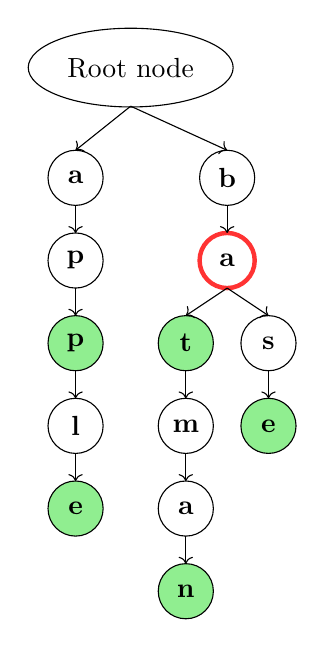
\begin{tikzpicture}[scale=0.7]
    % Vẽ hình elips chứa "Root node" tại tọa độ (0,0)
    \node[ellipse, draw, minimum width=2cm, minimum height=1cm] at (1,0) {Root node};
    
    % Vẽ vòng tròn chứa "a" tại (0,-2), không tô màu
     \fill[green] (0,-5) circle (0.5cm);
    \draw (0,-2) circle (0.5cm);
    \node at (0,-2) {\textbf{a}}; % Chữ "a" in đậm ở tâm vòng tròn
    \draw[->] (1,-0.7) -- (0,-1.5); % Mũi tên từ dưới "Root node" tới trên "a"
    
    % Vẽ vòng tròn chứa "p" thứ nhất tại (0,-3.5), không tô màu
    \draw (0,-3.5) circle (0.5cm);
    \node at (0,-3.5) {\textbf{p}}; % Chữ "p" in đậm ở tâm vòng tròn
    \draw[->] (0,-2.5) -- (0,-3); % Mũi tên từ dưới "a" tới trên "p"
    
    % Vẽ vòng tròn chứa "p" thứ hai tại (0,-5), không tô màu
    \draw (0,-5) circle (0.5cm);
    \node at (0,-5) {\textbf{p}}; % Chữ "p" in đậm ở tâm vòng tròn
    \draw[->] (0,-4) -- (0,-4.5); % Mũi tên từ dưới "p" trước tới trên "p"
    
    % Vẽ vòng tròn chứa "l" tại (0,-6.5), không tô màu
    \draw (0,-6.5) circle (0.5cm);
    \node at (0,-6.5) {\textbf{l}}; % Chữ "l" in đậm ở tâm vòng tròn
    \draw[->] (0,-5.5) -- (0,-6); % Mũi tên từ dưới "p" tới trên "l"
    
    % Vẽ vòng tròn chứa "e" tại (0,-8), tô màu xanh dương
    \fill[green] (0,-8) circle (0.5cm); % Tô nền màu xanh dương
    \draw (0,-8) circle (0.5cm); % Vẽ viền vòng tròn
    \node at (0,-8) {\textbf{e}}; % Chữ "e" in đậm ở tâm vòng tròn
    \draw[->] (0,-7) -- (0,-7.5); % Mũi tên từ dưới "l" tới trên "e"

    %b
 \draw (2.75,-2) circle (0.5cm);
\node at (2.75,-2) {\textbf{b}}; % Chữ "a" in đậm ở tâm vòng tròn
    \draw[->] (1,-0.7) -- (2.75,-1.5); % Mũi tên từ dưới "Root node" tới trên "a"
    %a
    \draw[red!80, ultra thick] (2.75,-3.5) circle (0.5cm);
    \node at (2.75,-3.5) {\textbf{a}}; % Chữ "a" in đậm ở tâm vòng tròn
    \draw[->] (2.75,-2.5) -- (2.75,-3); % Mũi tên từ dưới "Root node" tới trên
    %s
    \draw (3.5,-5) circle (0.5cm);
    \node at (3.5,-5) {\textbf{s}}; % Chữ "p" in đậm ở tâm vòng tròn
    \draw[->] (2.75,-4) -- (3.5,-4.5); % Mũi tên từ dưới "p" trước tới trên "p"
    %e
    \fill[green] (3.5,-6.5) circle (0.5cm);
     \draw (3.5,-6.5) circle (0.5cm);
    \node at (3.5,-6.5) {\textbf{e}}; % Chữ "l" in đậm ở tâm vòng tròn
    \draw[->] (3.5,-5.5) -- (3.5,-6); % Mũi tên từ dưới "p" tới trên "l"
    %t
    \fill[green] (2,-5) circle (0.5cm);
    \draw (2,-5) circle (0.5cm);
    \node at (2,-5) {\textbf{t}}; % Chữ "p" in đậm ở tâm vòng tròn
    \draw[->] (2.75,-4) -- (2,-4.5); % Mũi tên từ dưới "p" trước tới trên "p"
    %m
    \draw (2,-6.5) circle (0.5cm);
    \node at (2,-6.5) {\textbf{m}}; % Chữ "l" in đậm ở tâm vòng tròn
    \draw[->] (2,-5.5) -- (2,-6); % Mũi tên từ dưới "p" tới trên "l"
    %a
    \draw (02,-8) circle (0.5cm); % Vẽ viền vòng tròn
    \node at (02,-8) {\textbf{a}}; % Chữ "e" in đậm ở tâm vòng tròn
    \draw[->] (02,-7) -- (02,-7.5); % Mũi tên từ dưới "l" tới trên "e"
    %n
    \fill[green] (2,-9.5) circle (0.5cm); % Tô nền màu xanh dương
    \draw (02,-9.5) circle (0.5cm); % Vẽ viền vòng tròn
    \node at (02,-9.5) {\textbf{n}}; % Chữ "e" in đậm ở tâm vòng tròn
    \draw[->] (02,-8.5) -- (02,-9); % Mũi tên từ dưới "l" tới trên "e"
\end{tikzpicture}
    \end{center}
\end{frame}

\begin{frame}{Search "bat": TRUE}
    \begin{center}
            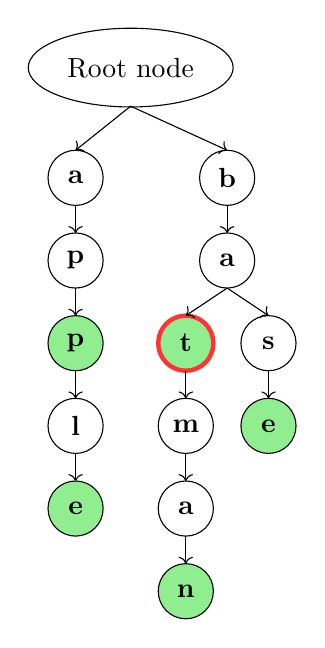
\begin{tikzpicture}[scale=0.7]
    % Vẽ hình elips chứa "Root node" tại tọa độ (0,0)
    \node[ellipse, draw, minimum width=2cm, minimum height=1cm] at (1,0) {Root node};
    
    % Vẽ vòng tròn chứa "a" tại (0,-2), không tô màu
     \fill[green] (0,-5) circle (0.5cm);
    \draw (0,-2) circle (0.5cm);
    \node at (0,-2) {\textbf{a}}; % Chữ "a" in đậm ở tâm vòng tròn
    \draw[->] (1,-0.7) -- (0,-1.5); % Mũi tên từ dưới "Root node" tới trên "a"
    
    % Vẽ vòng tròn chứa "p" thứ nhất tại (0,-3.5), không tô màu
    \draw (0,-3.5) circle (0.5cm);
    \node at (0,-3.5) {\textbf{p}}; % Chữ "p" in đậm ở tâm vòng tròn
    \draw[->] (0,-2.5) -- (0,-3); % Mũi tên từ dưới "a" tới trên "p"
    
    % Vẽ vòng tròn chứa "p" thứ hai tại (0,-5), không tô màu
    \draw (0,-5) circle (0.5cm);
    \node at (0,-5) {\textbf{p}}; % Chữ "p" in đậm ở tâm vòng tròn
    \draw[->] (0,-4) -- (0,-4.5); % Mũi tên từ dưới "p" trước tới trên "p"
    
    % Vẽ vòng tròn chứa "l" tại (0,-6.5), không tô màu
    \draw (0,-6.5) circle (0.5cm);
    \node at (0,-6.5) {\textbf{l}}; % Chữ "l" in đậm ở tâm vòng tròn
    \draw[->] (0,-5.5) -- (0,-6); % Mũi tên từ dưới "p" tới trên "l"
    
    % Vẽ vòng tròn chứa "e" tại (0,-8), tô màu xanh dương
    \fill[green] (0,-8) circle (0.5cm); % Tô nền màu xanh dương
    \draw (0,-8) circle (0.5cm); % Vẽ viền vòng tròn
    \node at (0,-8) {\textbf{e}}; % Chữ "e" in đậm ở tâm vòng tròn
    \draw[->] (0,-7) -- (0,-7.5); % Mũi tên từ dưới "l" tới trên "e"

    %b
 \draw (2.75,-2) circle (0.5cm);
\node at (2.75,-2) {\textbf{b}}; % Chữ "a" in đậm ở tâm vòng tròn
    \draw[->] (1,-0.7) -- (2.75,-1.5); % Mũi tên từ dưới "Root node" tới trên "a"
    %a
    \draw (2.75,-3.5) circle (0.5cm);
    \node at (2.75,-3.5) {\textbf{a}}; % Chữ "a" in đậm ở tâm vòng tròn
    \draw[->] (2.75,-2.5) -- (2.75,-3); % Mũi tên từ dưới "Root node" tới trên
    %s
    \draw (3.5,-5) circle (0.5cm);
    \node at (3.5,-5) {\textbf{s}}; % Chữ "p" in đậm ở tâm vòng tròn
    \draw[->] (2.75,-4) -- (3.5,-4.5); % Mũi tên từ dưới "p" trước tới trên "p"
    %e
    \fill[green] (3.5,-6.5) circle (0.5cm);
     \draw (3.5,-6.5) circle (0.5cm);
    \node at (3.5,-6.5) {\textbf{e}}; % Chữ "l" in đậm ở tâm vòng tròn
    \draw[->] (3.5,-5.5) -- (3.5,-6); % Mũi tên từ dưới "p" tới trên "l"
    %t
    \fill[green] (2,-5) circle (0.5cm);
    \draw[red!80, ultra thick] (2,-5) circle (0.5cm);
    \node at (2,-5) {\textbf{t}}; % Chữ "p" in đậm ở tâm vòng tròn
    \draw[->] (2.75,-4) -- (2,-4.5); % Mũi tên từ dưới "p" trước tới trên "p"
    %m
    \draw (2,-6.5) circle (0.5cm);
    \node at (2,-6.5) {\textbf{m}}; % Chữ "l" in đậm ở tâm vòng tròn
    \draw[->] (2,-5.5) -- (2,-6); % Mũi tên từ dưới "p" tới trên "l"
    %a
    \draw (02,-8) circle (0.5cm); % Vẽ viền vòng tròn
    \node at (02,-8) {\textbf{a}}; % Chữ "e" in đậm ở tâm vòng tròn
    \draw[->] (02,-7) -- (02,-7.5); % Mũi tên từ dưới "l" tới trên "e"
    %n
    \fill[green] (2,-9.5) circle (0.5cm); % Tô nền màu xanh dương
    \draw (02,-9.5) circle (0.5cm); % Vẽ viền vòng tròn
    \node at (02,-9.5) {\textbf{n}}; % Chữ "e" in đậm ở tâm vòng tròn
    \draw[->] (02,-8.5) -- (02,-9); % Mũi tên từ dưới "l" tới trên "e"
\end{tikzpicture}
    \end{center}
\end{frame}
\begin{frame}{Search "ba"}
    \begin{center}
            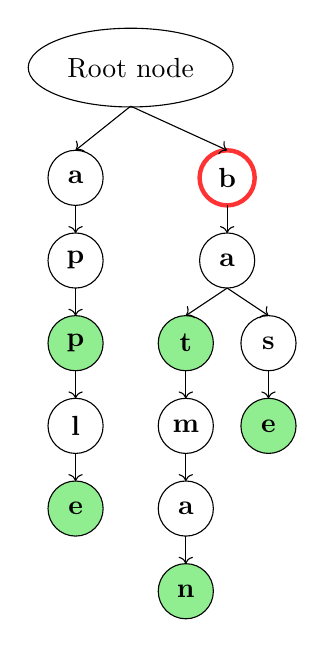
\begin{tikzpicture}[scale=0.7]
    % Vẽ hình elips chứa "Root node" tại tọa độ (0,0)
    \node[ellipse, draw, minimum width=2cm, minimum height=1cm] at (1,0) {Root node};
    
    % Vẽ vòng tròn chứa "a" tại (0,-2), không tô màu
     \fill[green] (0,-5) circle (0.5cm);
    \draw (0,-2) circle (0.5cm);
    \node at (0,-2) {\textbf{a}}; % Chữ "a" in đậm ở tâm vòng tròn
    \draw[->] (1,-0.7) -- (0,-1.5); % Mũi tên từ dưới "Root node" tới trên "a"
    
    % Vẽ vòng tròn chứa "p" thứ nhất tại (0,-3.5), không tô màu
    \draw (0,-3.5) circle (0.5cm);
    \node at (0,-3.5) {\textbf{p}}; % Chữ "p" in đậm ở tâm vòng tròn
    \draw[->] (0,-2.5) -- (0,-3); % Mũi tên từ dưới "a" tới trên "p"
    
    % Vẽ vòng tròn chứa "p" thứ hai tại (0,-5), không tô màu
    \draw (0,-5) circle (0.5cm);
    \node at (0,-5) {\textbf{p}}; % Chữ "p" in đậm ở tâm vòng tròn
    \draw[->] (0,-4) -- (0,-4.5); % Mũi tên từ dưới "p" trước tới trên "p"
    
    % Vẽ vòng tròn chứa "l" tại (0,-6.5), không tô màu
    \draw (0,-6.5) circle (0.5cm);
    \node at (0,-6.5) {\textbf{l}}; % Chữ "l" in đậm ở tâm vòng tròn
    \draw[->] (0,-5.5) -- (0,-6); % Mũi tên từ dưới "p" tới trên "l"
    
    % Vẽ vòng tròn chứa "e" tại (0,-8), tô màu xanh dương
    \fill[green] (0,-8) circle (0.5cm); % Tô nền màu xanh dương
    \draw (0,-8) circle (0.5cm); % Vẽ viền vòng tròn
    \node at (0,-8) {\textbf{e}}; % Chữ "e" in đậm ở tâm vòng tròn
    \draw[->] (0,-7) -- (0,-7.5); % Mũi tên từ dưới "l" tới trên "e"

    %b
\draw[red!80, ultra thick] (2.75,-2) circle (0.5cm);
\node at (2.75,-2) {\textbf{b}}; % Chữ "a" in đậm ở tâm vòng tròn
    \draw[->] (1,-0.7) -- (2.75,-1.5); % Mũi tên từ dưới "Root node" tới trên "a"
    %a
    \draw (2.75,-3.5) circle (0.5cm);
    \node at (2.75,-3.5) {\textbf{a}}; % Chữ "a" in đậm ở tâm vòng tròn
    \draw[->] (2.75,-2.5) -- (2.75,-3); % Mũi tên từ dưới "Root node" tới trên
    %s
    \draw (3.5,-5) circle (0.5cm);
    \node at (3.5,-5) {\textbf{s}}; % Chữ "p" in đậm ở tâm vòng tròn
    \draw[->] (2.75,-4) -- (3.5,-4.5); % Mũi tên từ dưới "p" trước tới trên "p"
    %e
    \fill[green] (3.5,-6.5) circle (0.5cm);
     \draw (3.5,-6.5) circle (0.5cm);
    \node at (3.5,-6.5) {\textbf{e}}; % Chữ "l" in đậm ở tâm vòng tròn
    \draw[->] (3.5,-5.5) -- (3.5,-6); % Mũi tên từ dưới "p" tới trên "l"
    %t
    \fill[green] (2,-5) circle (0.5cm);
    \draw (2,-5) circle (0.5cm);
    \node at (2,-5) {\textbf{t}}; % Chữ "p" in đậm ở tâm vòng tròn
    \draw[->] (2.75,-4) -- (2,-4.5); % Mũi tên từ dưới "p" trước tới trên "p"
    %m
    \draw (2,-6.5) circle (0.5cm);
    \node at (2,-6.5) {\textbf{m}}; % Chữ "l" in đậm ở tâm vòng tròn
    \draw[->] (2,-5.5) -- (2,-6); % Mũi tên từ dưới "p" tới trên "l"
    %a
    \draw (02,-8) circle (0.5cm); % Vẽ viền vòng tròn
    \node at (02,-8) {\textbf{a}}; % Chữ "e" in đậm ở tâm vòng tròn
    \draw[->] (02,-7) -- (02,-7.5); % Mũi tên từ dưới "l" tới trên "e"
    %n
    \fill[green] (2,-9.5) circle (0.5cm); % Tô nền màu xanh dương
    \draw (02,-9.5) circle (0.5cm); % Vẽ viền vòng tròn
    \node at (02,-9.5) {\textbf{n}}; % Chữ "e" in đậm ở tâm vòng tròn
    \draw[->] (02,-8.5) -- (02,-9); % Mũi tên từ dưới "l" tới trên "e"
\end{tikzpicture}
    \end{center}
\end{frame}
\begin{frame}{Search "ba": FALSE}
    \begin{center}
            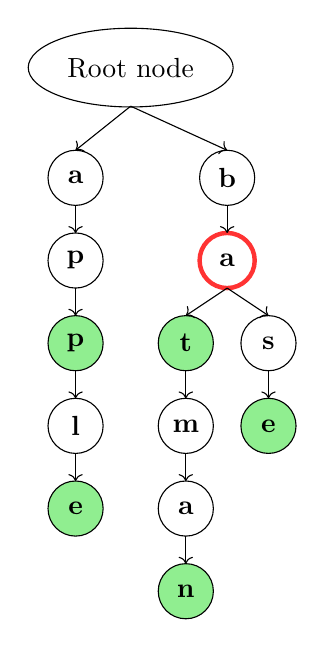
\begin{tikzpicture}[scale=0.7]
    % Vẽ hình elips chứa "Root node" tại tọa độ (0,0)
    \node[ellipse, draw, minimum width=2cm, minimum height=1cm] at (1,0) {Root node};
    
    % Vẽ vòng tròn chứa "a" tại (0,-2), không tô màu
     \fill[green] (0,-5) circle (0.5cm);
    \draw (0,-2) circle (0.5cm);
    \node at (0,-2) {\textbf{a}}; % Chữ "a" in đậm ở tâm vòng tròn
    \draw[->] (1,-0.7) -- (0,-1.5); % Mũi tên từ dưới "Root node" tới trên "a"
    
    % Vẽ vòng tròn chứa "p" thứ nhất tại (0,-3.5), không tô màu
    \draw (0,-3.5) circle (0.5cm);
    \node at (0,-3.5) {\textbf{p}}; % Chữ "p" in đậm ở tâm vòng tròn
    \draw[->] (0,-2.5) -- (0,-3); % Mũi tên từ dưới "a" tới trên "p"
    
    % Vẽ vòng tròn chứa "p" thứ hai tại (0,-5), không tô màu
    \draw (0,-5) circle (0.5cm);
    \node at (0,-5) {\textbf{p}}; % Chữ "p" in đậm ở tâm vòng tròn
    \draw[->] (0,-4) -- (0,-4.5); % Mũi tên từ dưới "p" trước tới trên "p"
    
    % Vẽ vòng tròn chứa "l" tại (0,-6.5), không tô màu
    \draw (0,-6.5) circle (0.5cm);
    \node at (0,-6.5) {\textbf{l}}; % Chữ "l" in đậm ở tâm vòng tròn
    \draw[->] (0,-5.5) -- (0,-6); % Mũi tên từ dưới "p" tới trên "l"
    
    % Vẽ vòng tròn chứa "e" tại (0,-8), tô màu xanh dương
    \fill[green] (0,-8) circle (0.5cm); % Tô nền màu xanh dương
    \draw (0,-8) circle (0.5cm); % Vẽ viền vòng tròn
    \node at (0,-8) {\textbf{e}}; % Chữ "e" in đậm ở tâm vòng tròn
    \draw[->] (0,-7) -- (0,-7.5); % Mũi tên từ dưới "l" tới trên "e"

    %b
 \draw (2.75,-2) circle (0.5cm);
\node at (2.75,-2) {\textbf{b}}; % Chữ "a" in đậm ở tâm vòng tròn
    \draw[->] (1,-0.7) -- (2.75,-1.5); % Mũi tên từ dưới "Root node" tới trên "a"
    %a
    \draw[red!80, ultra thick] (2.75,-3.5) circle (0.5cm);
    \node at (2.75,-3.5) {\textbf{a}}; % Chữ "a" in đậm ở tâm vòng tròn
    \draw[->] (2.75,-2.5) -- (2.75,-3); % Mũi tên từ dưới "Root node" tới trên
    %s
    \draw (3.5,-5) circle (0.5cm);
    \node at (3.5,-5) {\textbf{s}}; % Chữ "p" in đậm ở tâm vòng tròn
    \draw[->] (2.75,-4) -- (3.5,-4.5); % Mũi tên từ dưới "p" trước tới trên "p"
    %e
    \fill[green] (3.5,-6.5) circle (0.5cm);
     \draw (3.5,-6.5) circle (0.5cm);
    \node at (3.5,-6.5) {\textbf{e}}; % Chữ "l" in đậm ở tâm vòng tròn
    \draw[->] (3.5,-5.5) -- (3.5,-6); % Mũi tên từ dưới "p" tới trên "l"
    %t
    \fill[green] (2,-5) circle (0.5cm);
    \draw (2,-5) circle (0.5cm);
    \node at (2,-5) {\textbf{t}}; % Chữ "p" in đậm ở tâm vòng tròn
    \draw[->] (2.75,-4) -- (2,-4.5); % Mũi tên từ dưới "p" trước tới trên "p"
    %m
    \draw (2,-6.5) circle (0.5cm);
    \node at (2,-6.5) {\textbf{m}}; % Chữ "l" in đậm ở tâm vòng tròn
    \draw[->] (2,-5.5) -- (2,-6); % Mũi tên từ dưới "p" tới trên "l"
    %a
    \draw (02,-8) circle (0.5cm); % Vẽ viền vòng tròn
    \node at (02,-8) {\textbf{a}}; % Chữ "e" in đậm ở tâm vòng tròn
    \draw[->] (02,-7) -- (02,-7.5); % Mũi tên từ dưới "l" tới trên "e"
    %n
    \fill[green] (2,-9.5) circle (0.5cm); % Tô nền màu xanh dương
    \draw (02,-9.5) circle (0.5cm); % Vẽ viền vòng tròn
    \node at (02,-9.5) {\textbf{n}}; % Chữ "e" in đậm ở tâm vòng tròn
    \draw[->] (02,-8.5) -- (02,-9); % Mũi tên từ dưới "l" tới trên "e"
\end{tikzpicture}
    \end{center}
\end{frame}

\begin{frame}{Delete: O(L)}
    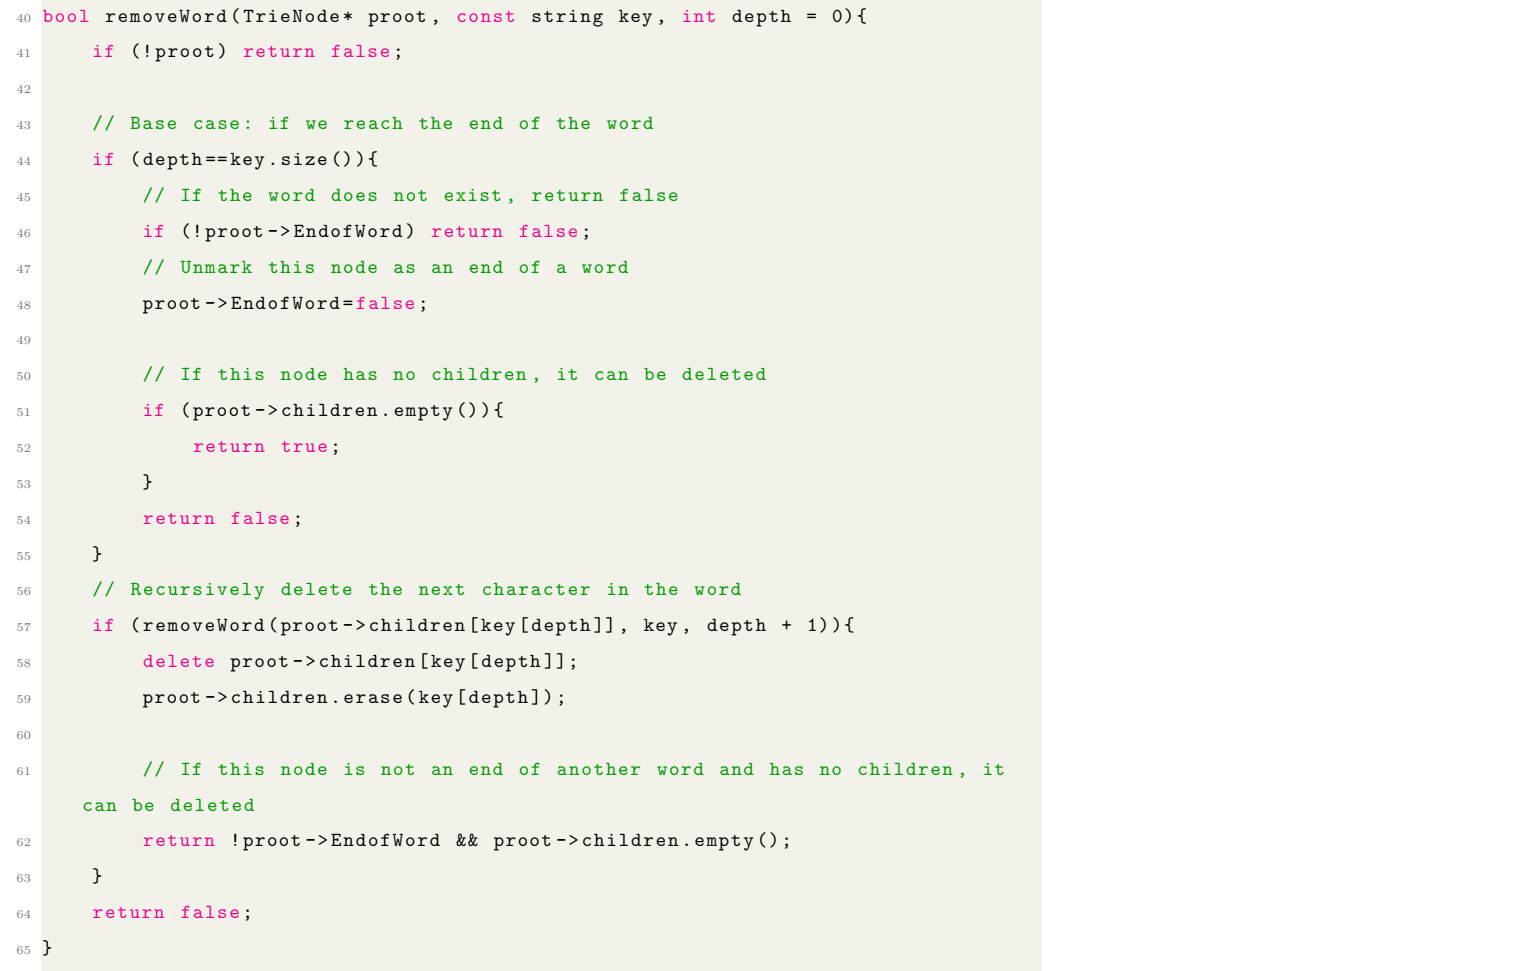
\includegraphics[scale=0.4]{se4.png}
\end{frame}
\begin{frame}{Delete "base"}
    \begin{center}
            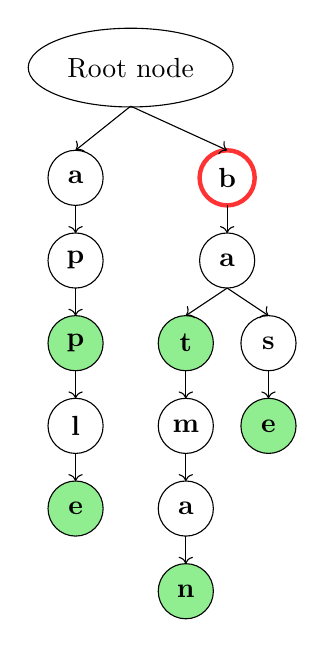
\begin{tikzpicture}[scale=0.7]
    % Vẽ hình elips chứa "Root node" tại tọa độ (0,0)
    \node[ellipse, draw, minimum width=2cm, minimum height=1cm] at (1,0) {Root node};
    
    % Vẽ vòng tròn chứa "a" tại (0,-2), không tô màu
     \fill[green] (0,-5) circle (0.5cm);
    \draw (0,-2) circle (0.5cm);
    \node at (0,-2) {\textbf{a}}; % Chữ "a" in đậm ở tâm vòng tròn
    \draw[->] (1,-0.7) -- (0,-1.5); % Mũi tên từ dưới "Root node" tới trên "a"
    
    % Vẽ vòng tròn chứa "p" thứ nhất tại (0,-3.5), không tô màu
    \draw (0,-3.5) circle (0.5cm);
    \node at (0,-3.5) {\textbf{p}}; % Chữ "p" in đậm ở tâm vòng tròn
    \draw[->] (0,-2.5) -- (0,-3); % Mũi tên từ dưới "a" tới trên "p"
    
    % Vẽ vòng tròn chứa "p" thứ hai tại (0,-5), không tô màu
    \draw (0,-5) circle (0.5cm);
    \node at (0,-5) {\textbf{p}}; % Chữ "p" in đậm ở tâm vòng tròn
    \draw[->] (0,-4) -- (0,-4.5); % Mũi tên từ dưới "p" trước tới trên "p"
    
    % Vẽ vòng tròn chứa "l" tại (0,-6.5), không tô màu
    \draw (0,-6.5) circle (0.5cm);
    \node at (0,-6.5) {\textbf{l}}; % Chữ "l" in đậm ở tâm vòng tròn
    \draw[->] (0,-5.5) -- (0,-6); % Mũi tên từ dưới "p" tới trên "l"
    
    % Vẽ vòng tròn chứa "e" tại (0,-8), tô màu xanh dương
    \fill[green] (0,-8) circle (0.5cm); % Tô nền màu xanh dương
    \draw (0,-8) circle (0.5cm); % Vẽ viền vòng tròn
    \node at (0,-8) {\textbf{e}}; % Chữ "e" in đậm ở tâm vòng tròn
    \draw[->] (0,-7) -- (0,-7.5); % Mũi tên từ dưới "l" tới trên "e"

    %b
\draw[red!80, ultra thick] (2.75,-2) circle (0.5cm);
\node at (2.75,-2) {\textbf{b}}; % Chữ "a" in đậm ở tâm vòng tròn
    \draw[->] (1,-0.7) -- (2.75,-1.5); % Mũi tên từ dưới "Root node" tới trên "a"
    %a
    \draw (2.75,-3.5) circle (0.5cm);
    \node at (2.75,-3.5) {\textbf{a}}; % Chữ "a" in đậm ở tâm vòng tròn
    \draw[->] (2.75,-2.5) -- (2.75,-3); % Mũi tên từ dưới "Root node" tới trên
    %s
    \draw (3.5,-5) circle (0.5cm);
    \node at (3.5,-5) {\textbf{s}}; % Chữ "p" in đậm ở tâm vòng tròn
    \draw[->] (2.75,-4) -- (3.5,-4.5); % Mũi tên từ dưới "p" trước tới trên "p"
    %e
    \fill[green] (3.5,-6.5) circle (0.5cm);
     \draw (3.5,-6.5) circle (0.5cm);
    \node at (3.5,-6.5) {\textbf{e}}; % Chữ "l" in đậm ở tâm vòng tròn
    \draw[->] (3.5,-5.5) -- (3.5,-6); % Mũi tên từ dưới "p" tới trên "l"
    %t
    \fill[green] (2,-5) circle (0.5cm);
    \draw (2,-5) circle (0.5cm);
    \node at (2,-5) {\textbf{t}}; % Chữ "p" in đậm ở tâm vòng tròn
    \draw[->] (2.75,-4) -- (2,-4.5); % Mũi tên từ dưới "p" trước tới trên "p"
    %m
    \draw (2,-6.5) circle (0.5cm);
    \node at (2,-6.5) {\textbf{m}}; % Chữ "l" in đậm ở tâm vòng tròn
    \draw[->] (2,-5.5) -- (2,-6); % Mũi tên từ dưới "p" tới trên "l"
    %a
    \draw (02,-8) circle (0.5cm); % Vẽ viền vòng tròn
    \node at (02,-8) {\textbf{a}}; % Chữ "e" in đậm ở tâm vòng tròn
    \draw[->] (02,-7) -- (02,-7.5); % Mũi tên từ dưới "l" tới trên "e"
    %n
    \fill[green] (2,-9.5) circle (0.5cm); % Tô nền màu xanh dương
    \draw (02,-9.5) circle (0.5cm); % Vẽ viền vòng tròn
    \node at (02,-9.5) {\textbf{n}}; % Chữ "e" in đậm ở tâm vòng tròn
    \draw[->] (02,-8.5) -- (02,-9); % Mũi tên từ dưới "l" tới trên "e"
\end{tikzpicture}
    \end{center}
\end{frame}
\begin{frame}{Delete "base"}
    \begin{center}
            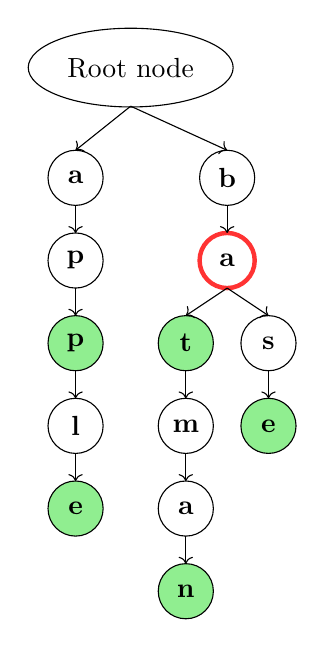
\begin{tikzpicture}[scale=0.7]
    % Vẽ hình elips chứa "Root node" tại tọa độ (0,0)
    \node[ellipse, draw, minimum width=2cm, minimum height=1cm] at (1,0) {Root node};
    
    % Vẽ vòng tròn chứa "a" tại (0,-2), không tô màu
     \fill[green] (0,-5) circle (0.5cm);
    \draw (0,-2) circle (0.5cm);
    \node at (0,-2) {\textbf{a}}; % Chữ "a" in đậm ở tâm vòng tròn
    \draw[->] (1,-0.7) -- (0,-1.5); % Mũi tên từ dưới "Root node" tới trên "a"
    
    % Vẽ vòng tròn chứa "p" thứ nhất tại (0,-3.5), không tô màu
    \draw (0,-3.5) circle (0.5cm);
    \node at (0,-3.5) {\textbf{p}}; % Chữ "p" in đậm ở tâm vòng tròn
    \draw[->] (0,-2.5) -- (0,-3); % Mũi tên từ dưới "a" tới trên "p"
    
    % Vẽ vòng tròn chứa "p" thứ hai tại (0,-5), không tô màu
    \draw (0,-5) circle (0.5cm);
    \node at (0,-5) {\textbf{p}}; % Chữ "p" in đậm ở tâm vòng tròn
    \draw[->] (0,-4) -- (0,-4.5); % Mũi tên từ dưới "p" trước tới trên "p"
    
    % Vẽ vòng tròn chứa "l" tại (0,-6.5), không tô màu
    \draw (0,-6.5) circle (0.5cm);
    \node at (0,-6.5) {\textbf{l}}; % Chữ "l" in đậm ở tâm vòng tròn
    \draw[->] (0,-5.5) -- (0,-6); % Mũi tên từ dưới "p" tới trên "l"
    
    % Vẽ vòng tròn chứa "e" tại (0,-8), tô màu xanh dương
    \fill[green] (0,-8) circle (0.5cm); % Tô nền màu xanh dương
    \draw (0,-8) circle (0.5cm); % Vẽ viền vòng tròn
    \node at (0,-8) {\textbf{e}}; % Chữ "e" in đậm ở tâm vòng tròn
    \draw[->] (0,-7) -- (0,-7.5); % Mũi tên từ dưới "l" tới trên "e"

    %b
 \draw (2.75,-2) circle (0.5cm);
\node at (2.75,-2) {\textbf{b}}; % Chữ "a" in đậm ở tâm vòng tròn
    \draw[->] (1,-0.7) -- (2.75,-1.5); % Mũi tên từ dưới "Root node" tới trên "a"
    %a
    \draw[red!80, ultra thick] (2.75,-3.5) circle (0.5cm);
    \node at (2.75,-3.5) {\textbf{a}}; % Chữ "a" in đậm ở tâm vòng tròn
    \draw[->] (2.75,-2.5) -- (2.75,-3); % Mũi tên từ dưới "Root node" tới trên
    %s
    \draw (3.5,-5) circle (0.5cm);
    \node at (3.5,-5) {\textbf{s}}; % Chữ "p" in đậm ở tâm vòng tròn
    \draw[->] (2.75,-4) -- (3.5,-4.5); % Mũi tên từ dưới "p" trước tới trên "p"
    %e
    \fill[green] (3.5,-6.5) circle (0.5cm);
     \draw (3.5,-6.5) circle (0.5cm);
    \node at (3.5,-6.5) {\textbf{e}}; % Chữ "l" in đậm ở tâm vòng tròn
    \draw[->] (3.5,-5.5) -- (3.5,-6); % Mũi tên từ dưới "p" tới trên "l"
    %t
    \fill[green] (2,-5) circle (0.5cm);
    \draw (2,-5) circle (0.5cm);
    \node at (2,-5) {\textbf{t}}; % Chữ "p" in đậm ở tâm vòng tròn
    \draw[->] (2.75,-4) -- (2,-4.5); % Mũi tên từ dưới "p" trước tới trên "p"
    %m
    \draw (2,-6.5) circle (0.5cm);
    \node at (2,-6.5) {\textbf{m}}; % Chữ "l" in đậm ở tâm vòng tròn
    \draw[->] (2,-5.5) -- (2,-6); % Mũi tên từ dưới "p" tới trên "l"
    %a
    \draw (02,-8) circle (0.5cm); % Vẽ viền vòng tròn
    \node at (02,-8) {\textbf{a}}; % Chữ "e" in đậm ở tâm vòng tròn
    \draw[->] (02,-7) -- (02,-7.5); % Mũi tên từ dưới "l" tới trên "e"
    %n
    \fill[green] (2,-9.5) circle (0.5cm); % Tô nền màu xanh dương
    \draw (02,-9.5) circle (0.5cm); % Vẽ viền vòng tròn
    \node at (02,-9.5) {\textbf{n}}; % Chữ "e" in đậm ở tâm vòng tròn
    \draw[->] (02,-8.5) -- (02,-9); % Mũi tên từ dưới "l" tới trên "e"
\end{tikzpicture}
    \end{center}
\end{frame}
\begin{frame}{Delete "base"}
    \begin{center}
            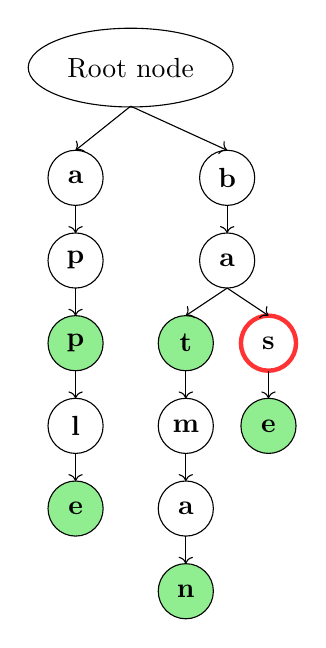
\begin{tikzpicture}[scale=0.7]
    % Vẽ hình elips chứa "Root node" tại tọa độ (0,0)
    \node[ellipse, draw, minimum width=2cm, minimum height=1cm] at (1,0) {Root node};
    
    % Vẽ vòng tròn chứa "a" tại (0,-2), không tô màu
     \fill[green] (0,-5) circle (0.5cm);
    \draw (0,-2) circle (0.5cm);
    \node at (0,-2) {\textbf{a}}; % Chữ "a" in đậm ở tâm vòng tròn
    \draw[->] (1,-0.7) -- (0,-1.5); % Mũi tên từ dưới "Root node" tới trên "a"
    
    % Vẽ vòng tròn chứa "p" thứ nhất tại (0,-3.5), không tô màu
    \draw (0,-3.5) circle (0.5cm);
    \node at (0,-3.5) {\textbf{p}}; % Chữ "p" in đậm ở tâm vòng tròn
    \draw[->] (0,-2.5) -- (0,-3); % Mũi tên từ dưới "a" tới trên "p"
    
    % Vẽ vòng tròn chứa "p" thứ hai tại (0,-5), không tô màu
    \draw (0,-5) circle (0.5cm);
    \node at (0,-5) {\textbf{p}}; % Chữ "p" in đậm ở tâm vòng tròn
    \draw[->] (0,-4) -- (0,-4.5); % Mũi tên từ dưới "p" trước tới trên "p"
    
    % Vẽ vòng tròn chứa "l" tại (0,-6.5), không tô màu
    \draw (0,-6.5) circle (0.5cm);
    \node at (0,-6.5) {\textbf{l}}; % Chữ "l" in đậm ở tâm vòng tròn
    \draw[->] (0,-5.5) -- (0,-6); % Mũi tên từ dưới "p" tới trên "l"
    
    % Vẽ vòng tròn chứa "e" tại (0,-8), tô màu xanh dương
    \fill[green] (0,-8) circle (0.5cm); % Tô nền màu xanh dương
    \draw (0,-8) circle (0.5cm); % Vẽ viền vòng tròn
    \node at (0,-8) {\textbf{e}}; % Chữ "e" in đậm ở tâm vòng tròn
    \draw[->] (0,-7) -- (0,-7.5); % Mũi tên từ dưới "l" tới trên "e"

    %b
 \draw (2.75,-2) circle (0.5cm);
\node at (2.75,-2) {\textbf{b}}; % Chữ "a" in đậm ở tâm vòng tròn
    \draw[->] (1,-0.7) -- (2.75,-1.5); % Mũi tên từ dưới "Root node" tới trên "a"
    %a
    \draw (2.75,-3.5) circle (0.5cm);
    \node at (2.75,-3.5) {\textbf{a}}; % Chữ "a" in đậm ở tâm vòng tròn
    \draw[->] (2.75,-2.5) -- (2.75,-3); % Mũi tên từ dưới "Root node" tới trên
    %s
    \draw[red!80, ultra thick] (3.5,-5) circle (0.5cm);
    \node at (3.5,-5) {\textbf{s}}; % Chữ "p" in đậm ở tâm vòng tròn
    \draw[->] (2.75,-4) -- (3.5,-4.5); % Mũi tên từ dưới "p" trước tới trên "p"
    %e
    \fill[green] (3.5,-6.5) circle (0.5cm);
     \draw (3.5,-6.5) circle (0.5cm);
    \node at (3.5,-6.5) {\textbf{e}}; % Chữ "l" in đậm ở tâm vòng tròn
    \draw[->] (3.5,-5.5) -- (3.5,-6); % Mũi tên từ dưới "p" tới trên "l"
    %t
    \fill[green] (2,-5) circle (0.5cm);
    \draw (2,-5) circle (0.5cm);
    \node at (2,-5) {\textbf{t}}; % Chữ "p" in đậm ở tâm vòng tròn
    \draw[->] (2.75,-4) -- (2,-4.5); % Mũi tên từ dưới "p" trước tới trên "p"
    %m
    \draw (2,-6.5) circle (0.5cm);
    \node at (2,-6.5) {\textbf{m}}; % Chữ "l" in đậm ở tâm vòng tròn
    \draw[->] (2,-5.5) -- (2,-6); % Mũi tên từ dưới "p" tới trên "l"
    %a
    \draw (02,-8) circle (0.5cm); % Vẽ viền vòng tròn
    \node at (02,-8) {\textbf{a}}; % Chữ "e" in đậm ở tâm vòng tròn
    \draw[->] (02,-7) -- (02,-7.5); % Mũi tên từ dưới "l" tới trên "e"
    %n
    \fill[green] (2,-9.5) circle (0.5cm); % Tô nền màu xanh dương
    \draw (02,-9.5) circle (0.5cm); % Vẽ viền vòng tròn
    \node at (02,-9.5) {\textbf{n}}; % Chữ "e" in đậm ở tâm vòng tròn
    \draw[->] (02,-8.5) -- (02,-9); % Mũi tên từ dưới "l" tới trên "e"
\end{tikzpicture}
    \end{center}
\end{frame}

\begin{frame}{Delete "base"}
    \begin{center}
            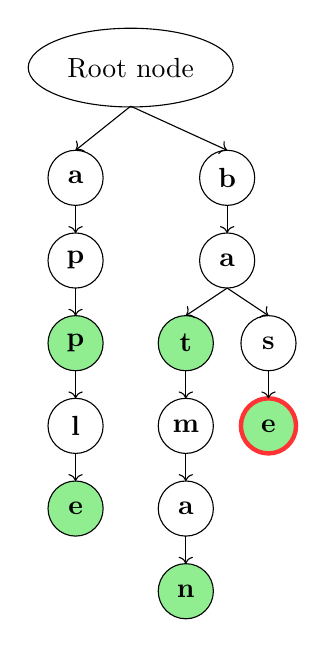
\begin{tikzpicture}[scale=0.7]
    % Vẽ hình elips chứa "Root node" tại tọa độ (0,0)
    \node[ellipse, draw, minimum width=2cm, minimum height=1cm] at (1,0) {Root node};
    
    % Vẽ vòng tròn chứa "a" tại (0,-2), không tô màu
     \fill[green] (0,-5) circle (0.5cm);
    \draw (0,-2) circle (0.5cm);
    \node at (0,-2) {\textbf{a}}; % Chữ "a" in đậm ở tâm vòng tròn
    \draw[->] (1,-0.7) -- (0,-1.5); % Mũi tên từ dưới "Root node" tới trên "a"
    
    % Vẽ vòng tròn chứa "p" thứ nhất tại (0,-3.5), không tô màu
    \draw (0,-3.5) circle (0.5cm);
    \node at (0,-3.5) {\textbf{p}}; % Chữ "p" in đậm ở tâm vòng tròn
    \draw[->] (0,-2.5) -- (0,-3); % Mũi tên từ dưới "a" tới trên "p"
    
    % Vẽ vòng tròn chứa "p" thứ hai tại (0,-5), không tô màu
    \draw (0,-5) circle (0.5cm);
    \node at (0,-5) {\textbf{p}}; % Chữ "p" in đậm ở tâm vòng tròn
    \draw[->] (0,-4) -- (0,-4.5); % Mũi tên từ dưới "p" trước tới trên "p"
    
    % Vẽ vòng tròn chứa "l" tại (0,-6.5), không tô màu
    \draw (0,-6.5) circle (0.5cm);
    \node at (0,-6.5) {\textbf{l}}; % Chữ "l" in đậm ở tâm vòng tròn
    \draw[->] (0,-5.5) -- (0,-6); % Mũi tên từ dưới "p" tới trên "l"
    
    % Vẽ vòng tròn chứa "e" tại (0,-8), tô màu xanh dương
    \fill[green] (0,-8) circle (0.5cm); % Tô nền màu xanh dương
    \draw (0,-8) circle (0.5cm); % Vẽ viền vòng tròn
    \node at (0,-8) {\textbf{e}}; % Chữ "e" in đậm ở tâm vòng tròn
    \draw[->] (0,-7) -- (0,-7.5); % Mũi tên từ dưới "l" tới trên "e"

    %b
 \draw (2.75,-2) circle (0.5cm);
\node at (2.75,-2) {\textbf{b}}; % Chữ "a" in đậm ở tâm vòng tròn
    \draw[->] (1,-0.7) -- (2.75,-1.5); % Mũi tên từ dưới "Root node" tới trên "a"
    %a
    \draw (2.75,-3.5) circle (0.5cm);
    \node at (2.75,-3.5) {\textbf{a}}; % Chữ "a" in đậm ở tâm vòng tròn
    \draw[->] (2.75,-2.5) -- (2.75,-3); % Mũi tên từ dưới "Root node" tới trên
    %s
    \draw (3.5,-5) circle (0.5cm);
    \node at (3.5,-5) {\textbf{s}}; % Chữ "p" in đậm ở tâm vòng tròn
    \draw[->] (2.75,-4) -- (3.5,-4.5); % Mũi tên từ dưới "p" trước tới trên "p"
    %e
    \fill[green] (3.5,-6.5) circle (0.5cm);
     \draw[red!80, ultra thick] (3.5,-6.5) circle (0.5cm);
    \node at (3.5,-6.5) {\textbf{e}}; % Chữ "l" in đậm ở tâm vòng tròn
    \draw[->] (3.5,-5.5) -- (3.5,-6); % Mũi tên từ dưới "p" tới trên "l"
    %t
    \fill[green] (2,-5) circle (0.5cm);
    \draw (2,-5) circle (0.5cm);
    \node at (2,-5) {\textbf{t}}; % Chữ "p" in đậm ở tâm vòng tròn
    \draw[->] (2.75,-4) -- (2,-4.5); % Mũi tên từ dưới "p" trước tới trên "p"
    %m
    \draw (2,-6.5) circle (0.5cm);
    \node at (2,-6.5) {\textbf{m}}; % Chữ "l" in đậm ở tâm vòng tròn
    \draw[->] (2,-5.5) -- (2,-6); % Mũi tên từ dưới "p" tới trên "l"
    %a
    \draw (02,-8) circle (0.5cm); % Vẽ viền vòng tròn
    \node at (02,-8) {\textbf{a}}; % Chữ "e" in đậm ở tâm vòng tròn
    \draw[->] (02,-7) -- (02,-7.5); % Mũi tên từ dưới "l" tới trên "e"
    %n
    \fill[green] (2,-9.5) circle (0.5cm); % Tô nền màu xanh dương
    \draw (02,-9.5) circle (0.5cm); % Vẽ viền vòng tròn
    \node at (02,-9.5) {\textbf{n}}; % Chữ "e" in đậm ở tâm vòng tròn
    \draw[->] (02,-8.5) -- (02,-9); % Mũi tên từ dưới "l" tới trên "e"
\end{tikzpicture}
    \end{center}
\end{frame}

\begin{frame}{Delete "base"}
    \begin{center}
            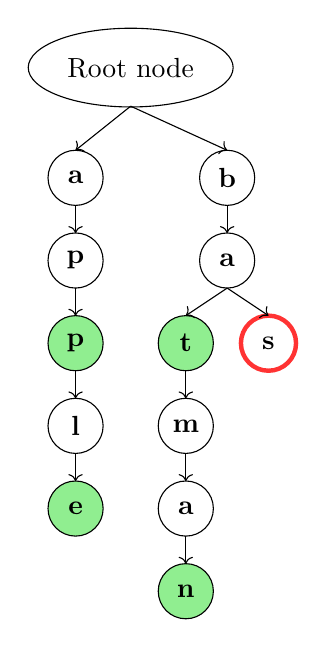
\begin{tikzpicture}[scale=0.7]
    % Vẽ hình elips chứa "Root node" tại tọa độ (0,0)
    \node[ellipse, draw, minimum width=2cm, minimum height=1cm] at (1,0) {Root node};
    
    % Vẽ vòng tròn chứa "a" tại (0,-2), không tô màu
     \fill[green] (0,-5) circle (0.5cm);
    \draw (0,-2) circle (0.5cm);
    \node at (0,-2) {\textbf{a}}; % Chữ "a" in đậm ở tâm vòng tròn
    \draw[->] (1,-0.7) -- (0,-1.5); % Mũi tên từ dưới "Root node" tới trên "a"
    
    % Vẽ vòng tròn chứa "p" thứ nhất tại (0,-3.5), không tô màu
    \draw (0,-3.5) circle (0.5cm);
    \node at (0,-3.5) {\textbf{p}}; % Chữ "p" in đậm ở tâm vòng tròn
    \draw[->] (0,-2.5) -- (0,-3); % Mũi tên từ dưới "a" tới trên "p"
    
    % Vẽ vòng tròn chứa "p" thứ hai tại (0,-5), không tô màu
    \draw (0,-5) circle (0.5cm);
    \node at (0,-5) {\textbf{p}}; % Chữ "p" in đậm ở tâm vòng tròn
    \draw[->] (0,-4) -- (0,-4.5); % Mũi tên từ dưới "p" trước tới trên "p"
    
    % Vẽ vòng tròn chứa "l" tại (0,-6.5), không tô màu
    \draw (0,-6.5) circle (0.5cm);
    \node at (0,-6.5) {\textbf{l}}; % Chữ "l" in đậm ở tâm vòng tròn
    \draw[->] (0,-5.5) -- (0,-6); % Mũi tên từ dưới "p" tới trên "l"
    
    % Vẽ vòng tròn chứa "e" tại (0,-8), tô màu xanh dương
    \fill[green] (0,-8) circle (0.5cm); % Tô nền màu xanh dương
    \draw (0,-8) circle (0.5cm); % Vẽ viền vòng tròn
    \node at (0,-8) {\textbf{e}}; % Chữ "e" in đậm ở tâm vòng tròn
    \draw[->] (0,-7) -- (0,-7.5); % Mũi tên từ dưới "l" tới trên "e"

    %b
 \draw (2.75,-2) circle (0.5cm);
\node at (2.75,-2) {\textbf{b}}; % Chữ "a" in đậm ở tâm vòng tròn
    \draw[->] (1,-0.7) -- (2.75,-1.5); % Mũi tên từ dưới "Root node" tới trên "a"
    %a
    \draw (2.75,-3.5) circle (0.5cm);
    \node at (2.75,-3.5) {\textbf{a}}; % Chữ "a" in đậm ở tâm vòng tròn
    \draw[->] (2.75,-2.5) -- (2.75,-3); % Mũi tên từ dưới "Root node" tới trên
    %s
    \draw[red!80, ultra thick] (3.5,-5) circle (0.5cm);
    \node at (3.5,-5) {\textbf{s}}; % Chữ "p" in đậm ở tâm vòng tròn
    \draw[->] (2.75,-4) -- (3.5,-4.5); % Mũi tên từ dưới "p" trước tới trên "p"
    %t
    \fill[green] (2,-5) circle (0.5cm);
    \draw (2,-5) circle (0.5cm);
    \node at (2,-5) {\textbf{t}}; % Chữ "p" in đậm ở tâm vòng tròn
    \draw[->] (2.75,-4) -- (2,-4.5); % Mũi tên từ dưới "p" trước tới trên "p"
    %m
    \draw (2,-6.5) circle (0.5cm);
    \node at (2,-6.5) {\textbf{m}}; % Chữ "l" in đậm ở tâm vòng tròn
    \draw[->] (2,-5.5) -- (2,-6); % Mũi tên từ dưới "p" tới trên "l"
    %a
    \draw (02,-8) circle (0.5cm); % Vẽ viền vòng tròn
    \node at (02,-8) {\textbf{a}}; % Chữ "e" in đậm ở tâm vòng tròn
    \draw[->] (02,-7) -- (02,-7.5); % Mũi tên từ dưới "l" tới trên "e"
    %n
    \fill[green] (2,-9.5) circle (0.5cm); % Tô nền màu xanh dương
    \draw (02,-9.5) circle (0.5cm); % Vẽ viền vòng tròn
    \node at (02,-9.5) {\textbf{n}}; % Chữ "e" in đậm ở tâm vòng tròn
    \draw[->] (02,-8.5) -- (02,-9); % Mũi tên từ dưới "l" tới trên "e"
\end{tikzpicture}
    \end{center}
\end{frame}

\begin{frame}{Delete "base"}
    \begin{center}
            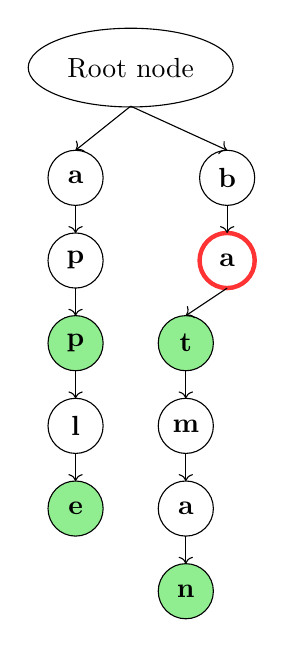
\begin{tikzpicture}[scale=0.7]
    % Vẽ hình elips chứa "Root node" tại tọa độ (0,0)
    \node[ellipse, draw, minimum width=2cm, minimum height=1cm] at (1,0) {Root node};
    
    % Vẽ vòng tròn chứa "a" tại (0,-2), không tô màu
     \fill[green] (0,-5) circle (0.5cm);
    \draw (0,-2) circle (0.5cm);
    \node at (0,-2) {\textbf{a}}; % Chữ "a" in đậm ở tâm vòng tròn
    \draw[->] (1,-0.7) -- (0,-1.5); % Mũi tên từ dưới "Root node" tới trên "a"
    
    % Vẽ vòng tròn chứa "p" thứ nhất tại (0,-3.5), không tô màu
    \draw (0,-3.5) circle (0.5cm);
    \node at (0,-3.5) {\textbf{p}}; % Chữ "p" in đậm ở tâm vòng tròn
    \draw[->] (0,-2.5) -- (0,-3); % Mũi tên từ dưới "a" tới trên "p"
    
    % Vẽ vòng tròn chứa "p" thứ hai tại (0,-5), không tô màu
    \draw (0,-5) circle (0.5cm);
    \node at (0,-5) {\textbf{p}}; % Chữ "p" in đậm ở tâm vòng tròn
    \draw[->] (0,-4) -- (0,-4.5); % Mũi tên từ dưới "p" trước tới trên "p"
    
    % Vẽ vòng tròn chứa "l" tại (0,-6.5), không tô màu
    \draw (0,-6.5) circle (0.5cm);
    \node at (0,-6.5) {\textbf{l}}; % Chữ "l" in đậm ở tâm vòng tròn
    \draw[->] (0,-5.5) -- (0,-6); % Mũi tên từ dưới "p" tới trên "l"
    
    % Vẽ vòng tròn chứa "e" tại (0,-8), tô màu xanh dương
    \fill[green] (0,-8) circle (0.5cm); % Tô nền màu xanh dương
    \draw (0,-8) circle (0.5cm); % Vẽ viền vòng tròn
    \node at (0,-8) {\textbf{e}}; % Chữ "e" in đậm ở tâm vòng tròn
    \draw[->] (0,-7) -- (0,-7.5); % Mũi tên từ dưới "l" tới trên "e"

    %b
 \draw (2.75,-2) circle (0.5cm);
\node at (2.75,-2) {\textbf{b}}; % Chữ "a" in đậm ở tâm vòng tròn
    \draw[->] (1,-0.7) -- (2.75,-1.5); % Mũi tên từ dưới "Root node" tới trên "a"
    %a
    \draw[red!80, ultra thick]  (2.75,-3.5) circle (0.5cm);
    \node at (2.75,-3.5) {\textbf{a}}; % Chữ "a" in đậm ở tâm vòng tròn
    \draw[->] (2.75,-2.5) -- (2.75,-3); % Mũi tên từ dưới "Root node" tới trên
    %t
    \fill[green] (2,-5) circle (0.5cm);
    \draw (2,-5) circle (0.5cm);
    \node at (2,-5) {\textbf{t}}; % Chữ "p" in đậm ở tâm vòng tròn
    \draw[->] (2.75,-4) -- (2,-4.5); % Mũi tên từ dưới "p" trước tới trên "p"
    %m
    \draw (2,-6.5) circle (0.5cm);
    \node at (2,-6.5) {\textbf{m}}; % Chữ "l" in đậm ở tâm vòng tròn
    \draw[->] (2,-5.5) -- (2,-6); % Mũi tên từ dưới "p" tới trên "l"
    %a
    \draw (02,-8) circle (0.5cm); % Vẽ viền vòng tròn
    \node at (02,-8) {\textbf{a}}; % Chữ "e" in đậm ở tâm vòng tròn
    \draw[->] (02,-7) -- (02,-7.5); % Mũi tên từ dưới "l" tới trên "e"
    %n
    \fill[green] (2,-9.5) circle (0.5cm); % Tô nền màu xanh dương
    \draw (02,-9.5) circle (0.5cm); % Vẽ viền vòng tròn
    \node at (02,-9.5) {\textbf{n}}; % Chữ "e" in đậm ở tâm vòng tròn
    \draw[->] (02,-8.5) -- (02,-9); % Mũi tên từ dưới "l" tới trên "e"
\end{tikzpicture}
    \end{center}
\end{frame}
\begin{frame}{Insert "batman"}
\begin{center}
    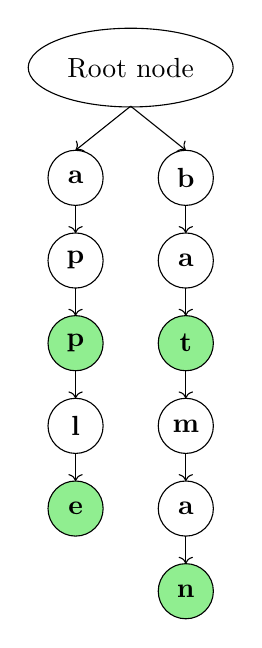
\begin{tikzpicture}[scale=0.7]
    % Vẽ hình elips chứa "Root node" tại tọa độ (0,0)
    \node[ellipse, draw, minimum width=2cm, minimum height=1cm] at (1,0) {Root node};
    
    % Vẽ vòng tròn chứa "a" tại (0,-2), không tô màu
     \fill[green] (0,-5) circle (0.5cm);
    \draw (0,-2) circle (0.5cm);
    \node at (0,-2) {\textbf{a}}; % Chữ "a" in đậm ở tâm vòng tròn
    \draw[->] (1,-0.7) -- (0,-1.5); % Mũi tên từ dưới "Root node" tới trên "a"
    
    % Vẽ vòng tròn chứa "p" thứ nhất tại (0,-3.5), không tô màu
    \draw (0,-3.5) circle (0.5cm);
    \node at (0,-3.5) {\textbf{p}}; % Chữ "p" in đậm ở tâm vòng tròn
    \draw[->] (0,-2.5) -- (0,-3); % Mũi tên từ dưới "a" tới trên "p"
    
    % Vẽ vòng tròn chứa "p" thứ hai tại (0,-5), không tô màu
    \draw (0,-5) circle (0.5cm);
    \node at (0,-5) {\textbf{p}}; % Chữ "p" in đậm ở tâm vòng tròn
    \draw[->] (0,-4) -- (0,-4.5); % Mũi tên từ dưới "p" trước tới trên "p"
    
    % Vẽ vòng tròn chứa "l" tại (0,-6.5), không tô màu
    \draw (0,-6.5) circle (0.5cm);
    \node at (0,-6.5) {\textbf{l}}; % Chữ "l" in đậm ở tâm vòng tròn
    \draw[->] (0,-5.5) -- (0,-6); % Mũi tên từ dưới "p" tới trên "l"
    
    % Vẽ vòng tròn chứa "e" tại (0,-8), tô màu xanh dương
    \fill[green] (0,-8) circle (0.5cm); % Tô nền màu xanh dương
    \draw (0,-8) circle (0.5cm); % Vẽ viền vòng tròn
    \node at (0,-8) {\textbf{e}}; % Chữ "e" in đậm ở tâm vòng tròn
    \draw[->] (0,-7) -- (0,-7.5); % Mũi tên từ dưới "l" tới trên "e"

    %b
    \draw (2,-2) circle (0.5cm);
    \node at (2,-2) {\textbf{b}}; % Chữ "a" in đậm ở tâm vòng tròn
    \draw[->] (1,-0.7) -- (2,-1.5); % Mũi tên từ dưới "Root node" tới trên "a"
    %a
    \draw (2,-3.5) circle (0.5cm);
    \node at (2,-3.5) {\textbf{a}}; % Chữ "a" in đậm ở tâm vòng tròn
    \draw[->] (2,-2.5) -- (2,-3); % Mũi tên từ dưới "Root node" tới trên "a"
    %t
    \fill[green] (2,-5) circle (0.5cm);
    \draw (2,-5) circle (0.5cm);
    \node at (2,-5) {\textbf{t}}; % Chữ "p" in đậm ở tâm vòng tròn
    \draw[->] (2,-4) -- (2,-4.5); % Mũi tên từ dưới "p" trước tới trên "p"
    %m
    \draw (2,-6.5) circle (0.5cm);
    \node at (2,-6.5) {\textbf{m}}; % Chữ "l" in đậm ở tâm vòng tròn
    \draw[->] (2,-5.5) -- (2,-6); % Mũi tên từ dưới "p" tới trên "l"
    %a
    \draw (02,-8) circle (0.5cm); % Vẽ viền vòng tròn
    \node at (02,-8) {\textbf{a}}; % Chữ "e" in đậm ở tâm vòng tròn
    \draw[->] (02,-7) -- (02,-7.5); % Mũi tên từ dưới "l" tới trên "e"
    %n
    \fill[green] (2,-9.5) circle (0.5cm); % Tô nền màu xanh dương
    \draw (02,-9.5) circle (0.5cm); % Vẽ viền vòng tròn
    \node at (02,-9.5) {\textbf{n}}; % Chữ "e" in đậm ở tâm vòng tròn
    \draw[->] (02,-8.5) -- (02,-9); % Mũi tên từ dưới "l" tới trên "e"
\end{tikzpicture}
\end{center}
\end{frame}

\begin{frame}{Space Complexity}
    $O(N * M)$, where $N$ is the number of words and $M$ is the average word length. Each character across all words requires a node (or a slot in a dictionary/array), causing the space to scale with the total number of characters stored.
\end{frame}

\section{Applications}


\begin{frame}{Competitive Programming Applications}
    \textbf{1) String Processing}
\begin{itemize}
    \item String Matching and Dictionary Problems
    \item Suffix Trie for Pattern Searching
\end{itemize}

\textbf{2) Optimization and Searching}
\begin{itemize}
    \item Longest Prefix Matching Algorithm
    \item Counting Unique Substrings (Suffix Trie)
    \item XOR Maximization
\end{itemize}

\textbf{3) Dynamic Programming and Optimization}
\begin{itemize}
    \item Dynamic Programming with Trie
    \begin{itemize}
        \item Word Break Problem: Determines if a string can be segmented into valid words using DP + Trie.
        \item String DP Problems: Optimization for finding shortest unique prefixes.
    \end{itemize}
\end{itemize}
\end{frame}



\begin{frame}{Practical Applications}
    \textbf{1) Search and Retrieval}
\begin{itemize}
    \item Search Engines and Autocomplete.
    \begin{itemize}
        \item Google search and keyboards use Trie-based approaches for fast suggestions.
        \item Helps in auto-correct and word prediction in text input.
        \end{itemize}
    \item Dictionary
\end{itemize}

\textbf{2) Data Compression and Encoding}
\begin{itemize}
    \item Compression and Encoding
    \begin{itemize}
        \item Used in Huffman Coding to build prefix-free encoding schemes.
        \item Some Lempel-Ziv compression algorithms use Tries for efficient substring matching.
    \end{itemize}
\end{itemize}
\end{frame}
\begin{frame}{Practical Applications}
    \textbf{3) Networking and Security}
\begin{itemize}
    \item Network Routing and IP Lookup
    \begin{itemize}
        \item Trie-based structures optimize IP routing tables for efficient packet forwarding.
        \item Used in firewall rule matching and domain name resolution.
    \end{itemize}
\end{itemize}

\textbf{4) Natural Language Processing (NLP)}
\begin{itemize}
    \item Helps in word segmentation for text analysis.
    \item Used in AI chatbots for fast word lookups and pattern recognition.
\end{itemize}

\end{frame}


\section{Advantages and Disadvantages of Trie}

\begin{frame}{Advantages}
    \begin{itemize}[label=$\star$]
    \item Efficient for searching, inserting and deleting words in the time complexity $O(L)$, where $L$ is the length of the word (faster than both the hash tables and the binary search tree in prefix matching).
    \item Supports prefix-based operations efficiently, making it useful for autocomplete and dictionary implementations.
    \item Can handle a large number of words without collisions, unlike hash tables.
    \item Provides lexicographical sorting of stored words naturally.
    \item Useful in applications such as IP routing, search engines, and natural language processing.
    \item More space efficient compare to binary search tree.
\end{itemize}
\end{frame}

\begin{frame}{Disadvantages}
    \begin{itemize}[label=$\star$]
    \item High memory consumption due to storing multiple nodes for each character.
    \item Not space-efficient when storing a small number of words compared to hash tables.
    \item Can be slower than hash tables for exact word searches since hashing has average $O(1)$ lookup time.
    \item Requires extra implementation effort compared to simpler data structures.
\end{itemize}

\end{frame}

\section{Quizzes}
\begin{frame}{1. Trie is also known as}
    
    \begin{enumerate}[label=\alph*.]
    \item Prefix Tree
    \item Treap
    \item Binomial Tree
    \item 2-3 Tree
\end{enumerate}
\end{frame}
\begin{frame}{1. Trie is also known as}
    \begin{enumerate}[label=\alph*.]
    \item \textbf{Prefix Tree}
    \item Treap
    \item Binomial Tree
    \item 2-3 Tree
\end{enumerate}
\end{frame}
\begin{frame}{ What traversal over trie gives the lexicographical sorting of the set of the strings?}
    \begin{enumerate}[label=\alph*.]
        \item Postorder
        \item Preorders
        \item Inorder
        \item Level order
    \end{enumerate}
\end{frame}
\begin{frame}{ What traversal over trie gives the lexicographical sorting of the set of the strings?}
    \begin{enumerate}[label=\alph*.]
        \item Postorder
        \item \textbf{Preorders}
        \item Inorder
        \item Level order
    \end{enumerate}
\end{frame}
\begin{frame}{Which of the following is not true?}
     \begin{enumerate}[label=\alph*.]
        \item Trie requires less storage space than hashing
        \item Trie allows listing of all the words with same prefix
        \item Tries are collision free
        \item Trie is also known as prefix tree
     \end{enumerate}
\end{frame}
\begin{frame}{Which of the following is not true?}
     \begin{enumerate}[label=\alph*.]
        \item \textbf{Trie requires less storage space than hashing}
        \item Trie allows listing of all the words with same prefix
        \item Tries are collision free
        \item Trie is also known as prefix tree
     \end{enumerate}
\end{frame}
\begin{frame}{What can be the maximum depth of the trie with $n$ strings and $m$ as the maximum string the length?}
    \begin{enumerate}[label=\alph*.]
    \item $\log_2(n)$ 
    \item $\log_2(m)$
    \item n
    \item m
    \end{enumerate}
\end{frame}
\begin{frame}{What can be the maximum depth of the trie with $n$ strings and $m$ as the maximum sting the length?}
    \begin{enumerate}[label=\alph*.]
    \item $\log_2(n)$ 
    \item $\log_2(m)$
    \item n
    \item m
    \end{enumerate}
\end{frame}
\begin{frame}{Which of the following is true about the trie?}
    \begin{enumerate}[label=\alph*.]
    \item root is letter 'a'
    \item path from root to the leaf yields the string
    \item children of nodes are randomly ordered
    \item each node stores the associated keys
    \end{enumerate}
\end{frame}
\begin{frame}{Which of the following is true about the trie?}
    \begin{enumerate}[label=\alph*.]
    \item root is letter 'a'
    \item \textbf{path from root to the leaf yields the string}
    \item children of nodes are randomly ordered
    \item each node stores the associated keys
    \end{enumerate}
\end{frame}

\end{document}